\section{Supporting Simulations with OpenFOAM}

\subsection{Case Setup GUI: \texttt{isofCaseBuilder}}

\subsection{Execution Monitor GUI: \texttt{isofExecutionManager}}

\subsection{Tabular Output Data Plot: \texttt{isofPlotTabular}}

\subsection{Clean OpenFOAM Case Directories: \texttt{isofCleanCase}}
\label{sec:isofcleancase}





\subsection{Common Tasks in the Context of OpenFOAM Simulations}

\subsubsection{Controlling and Checking Running OpenFOAM Case Which Were Generated by InsightCAE}

OpenFOAM cases which were generated by InsightCAE are enhanced with a number of additional features.
These are utilized by the workbench frontend but can also be used to modify cases manually.

\paragraph{Trigger Output Independently from the Configured Output Interval}
\label{par:trigger_output_of}
\label{par:wnow}

The solver monitors the files in its case directory.
If it finds a file named \verb!wnow!, immediate output is triggered and this signal file is removed by the solver.

This feature can be used to inspect the solution at any time while the solver is running using Paraview.

The file can e.g. created from the terminal:

\begin{lstlisting}
$ touch wnow
\end{lstlisting}

Note: you might need to change to working directory to the case directory first.

\paragraph{Trigger Immediate Output and Stop Solver Afterwards Without Raising an Error}
\label{par:wnowandstop}
The solver monitors the files in its case directory.
If it finds a file named \verb!wnowandstop!, immediate output is triggered, this signal file is removed by the solver and the solvers.

This feature can be used e.g. to gracefully and a solver run which is converged and the convergence is recognized by the user but not yet by the convergence monitoring feature of InsightCAE.

The file can e.g. created from the terminal:

\begin{lstlisting}
$ touch wnowandstop
\end{lstlisting}

Note: you might need to change to working directory to the case directory first.



\paragraph{Inspecting a Running Case Using Paraview}
\label{par:isPVpy}

Some of the relevant numerical figures of a case are displayed in live updated charts in the GUI.
But it is a very good habit to check the mesh and also the solution as soon as possible and well before valuable computing resource are wasted to compute inadequate solutions on bad meshes.
If problems with the mesh or the solutions become obvious, it is possible to stop the analysis (e.g. by the "Kill" button in the workbench or by pressing CTRL+C in the terminal, where the analyze command line tool is running) and revise the settings.

The OpenFOAM cases can be loaded into Paraview as soon as they were created by one of the InsightCAE modules.
It is perfectly possible to do this while the solver is running.
It is also possible to trigger extra output if it is not yet available (see first paragraph of this section).


\begin{itemize}
\item 
When output\footnote{Data of every output time instance is stored in a so-called time directory. These are directories in the case directory whose names are just numbers. The number correspond to the simulation time to which the data belongs. For a parallel run, these directories are created in the processor directories below the case directory and for a serial run, they are found directly in the top level case directory.} is there, Paravie w is best launched by InsightCAE's wrapper script \verb!isPV.py!:

\begin{lstlisting}
$ isPV.py
\end{lstlisting}

Note: you might need to change to working directory to the case directory first.

\item
The wrapper automatically inserts the OpenFOAM case reader source into Paraviews' visualization pipeline.
You should consider the following settings:
\begin{enumerate}
\item Select at least all the mesh regions, which you would like to inspect. You can later filter out subsets of mesh regions. So it is ok, to select all.
\item Select the case type: either 
\begin{itemize}
\item "Reconstructed Case", if you performed a serial run or if the output has been already reconstructed from the processor directories (usually done for the last time step during the evaluation step)
\item "Decomposed Case", if you want to monitor a parallel run.
\end{itemize}
\end{enumerate}

When all settings are right, click on "Apply".

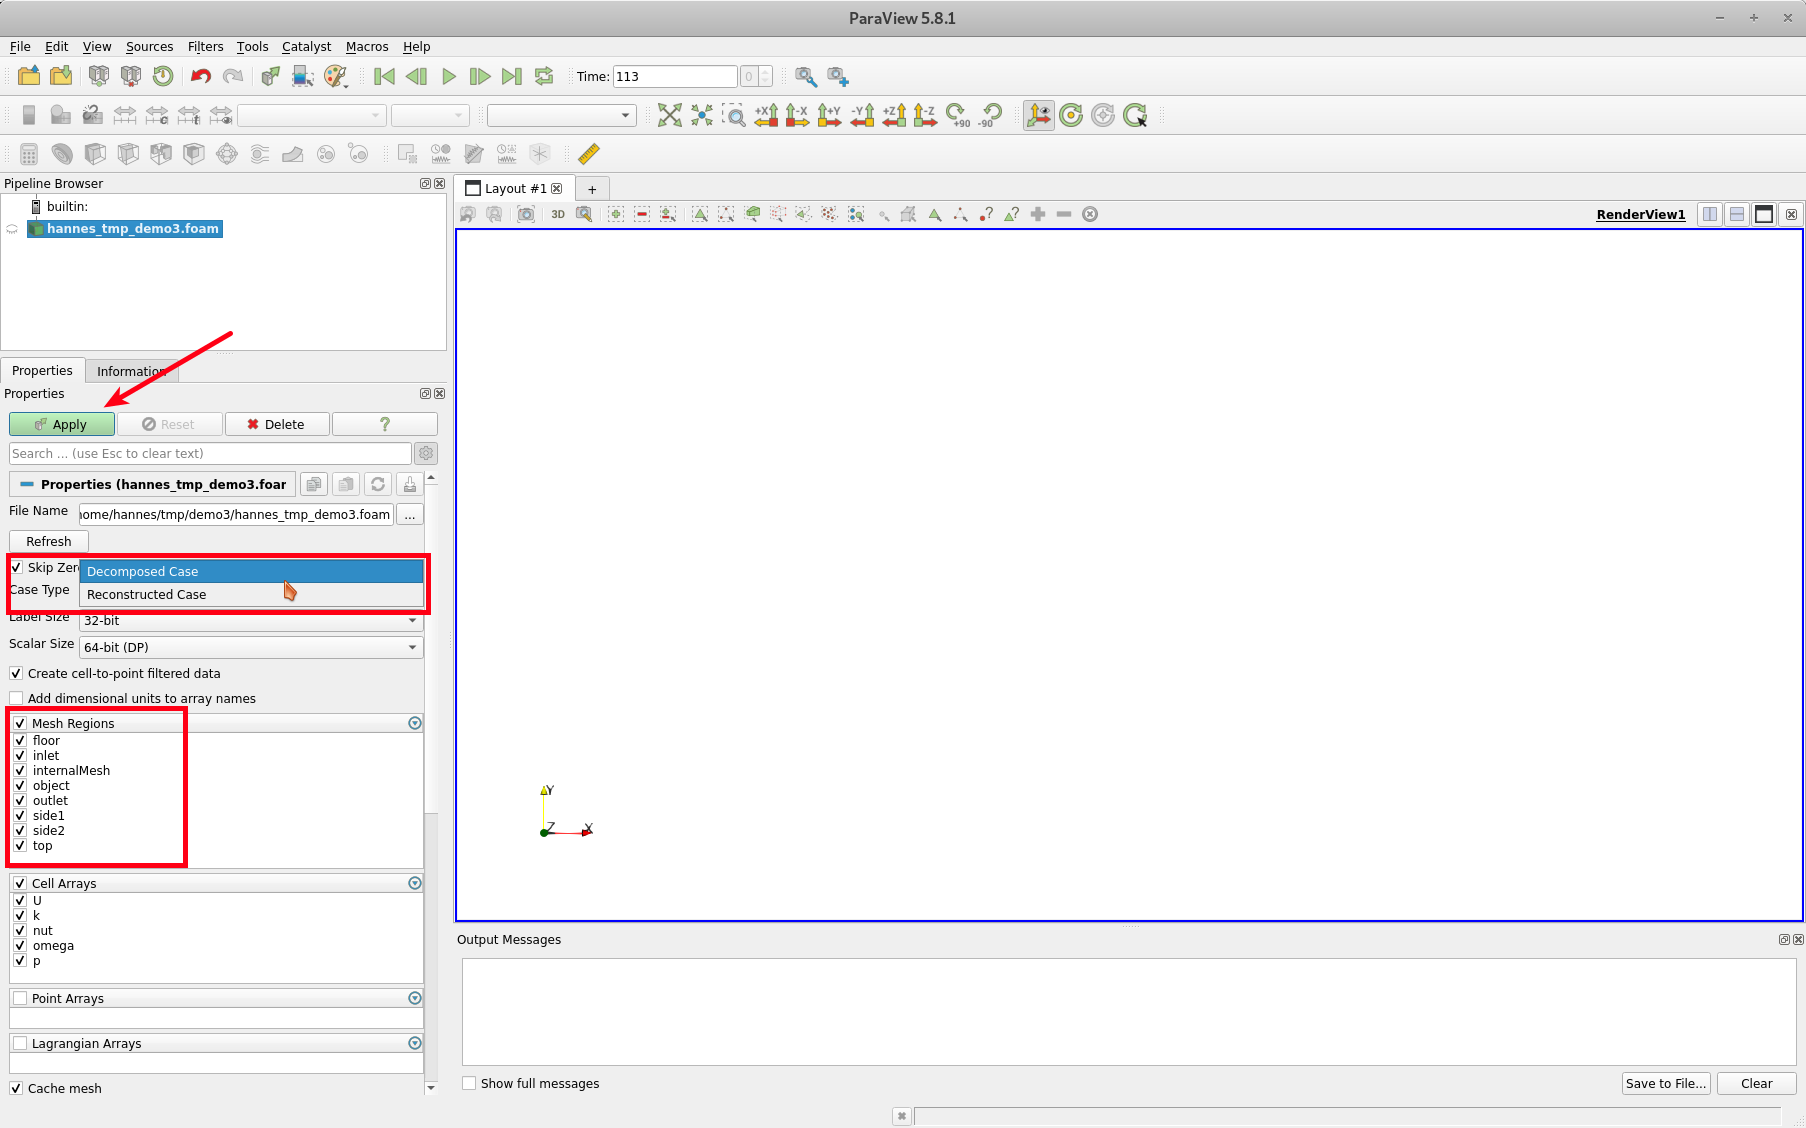
\includegraphics[width=0.75\linewidth]{figs/paraview_of/paraview_load_case}

\item
Next, jump to the latest time step:

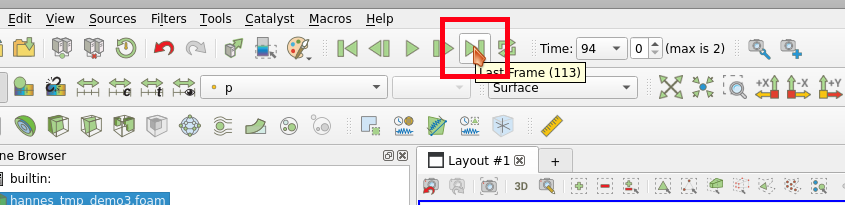
\includegraphics[width=0.75\linewidth]{figs/paraview_of/jump_to_latest_timestep}

\item Now, the scene can be set up using all the Paraview filters\footnote{see \url{https://www.paraview.org/paraview-guide/} for Paraview's User Guide. It can be viewed online.}.

Often, fields on boundary regions (e.g. walls) are of interest.
These can be extracted using the "Extract Block" filter.
To apply this filter, select from the menu \menu{Filters>Alphabetical>Extract Block}.
Make sure that the OpenFOAM case source is selected in the pipeline browser when the filter is added.
When all the boundaries of interest are selected, click on "Apply".

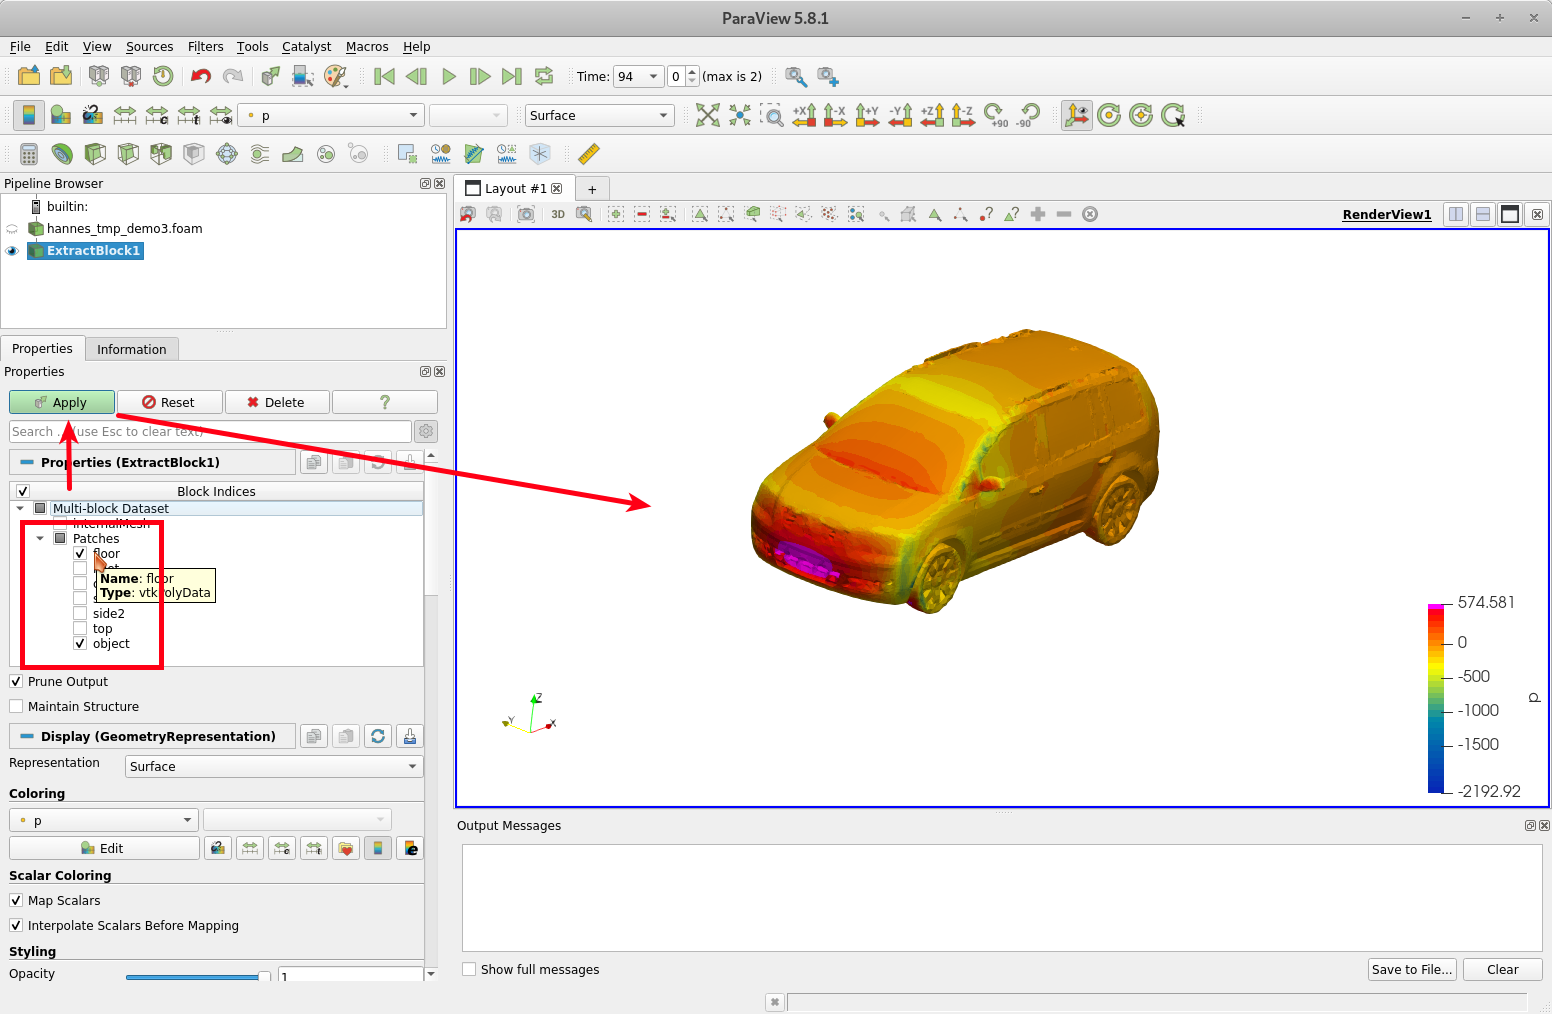
\includegraphics[width=0.75\linewidth]{figs/paraview_of/paraview_extract_block}

\end{itemize}



\subsubsection{Meshing}



\paragraph{Extraction of Feature Edges from STL Geometries}

Features edges can be extracted automatically from STLs. 
They are usually found by looking at the angle between neighbouring triangular facets.
This methods is usually automatically applied either in snapphyHexMesh itself or within InsightCAE's workflows.
This method works nicely for edges between planar surfaces.
Though it fails e.g. for rounded edges like leading and trailing edges of propellers and foils.
In such cases, it is required to extract feature edges manually and feed them into the meshing process.

Here, it is described how to extract feature curves using the open source software Blender\footnote{\url{https://www.blender.org/}}.
The following steps are required:
\begin{enumerate}
\item Import the geometry into Blender

select in menu \menu{File>Import>STL (*.stl)}

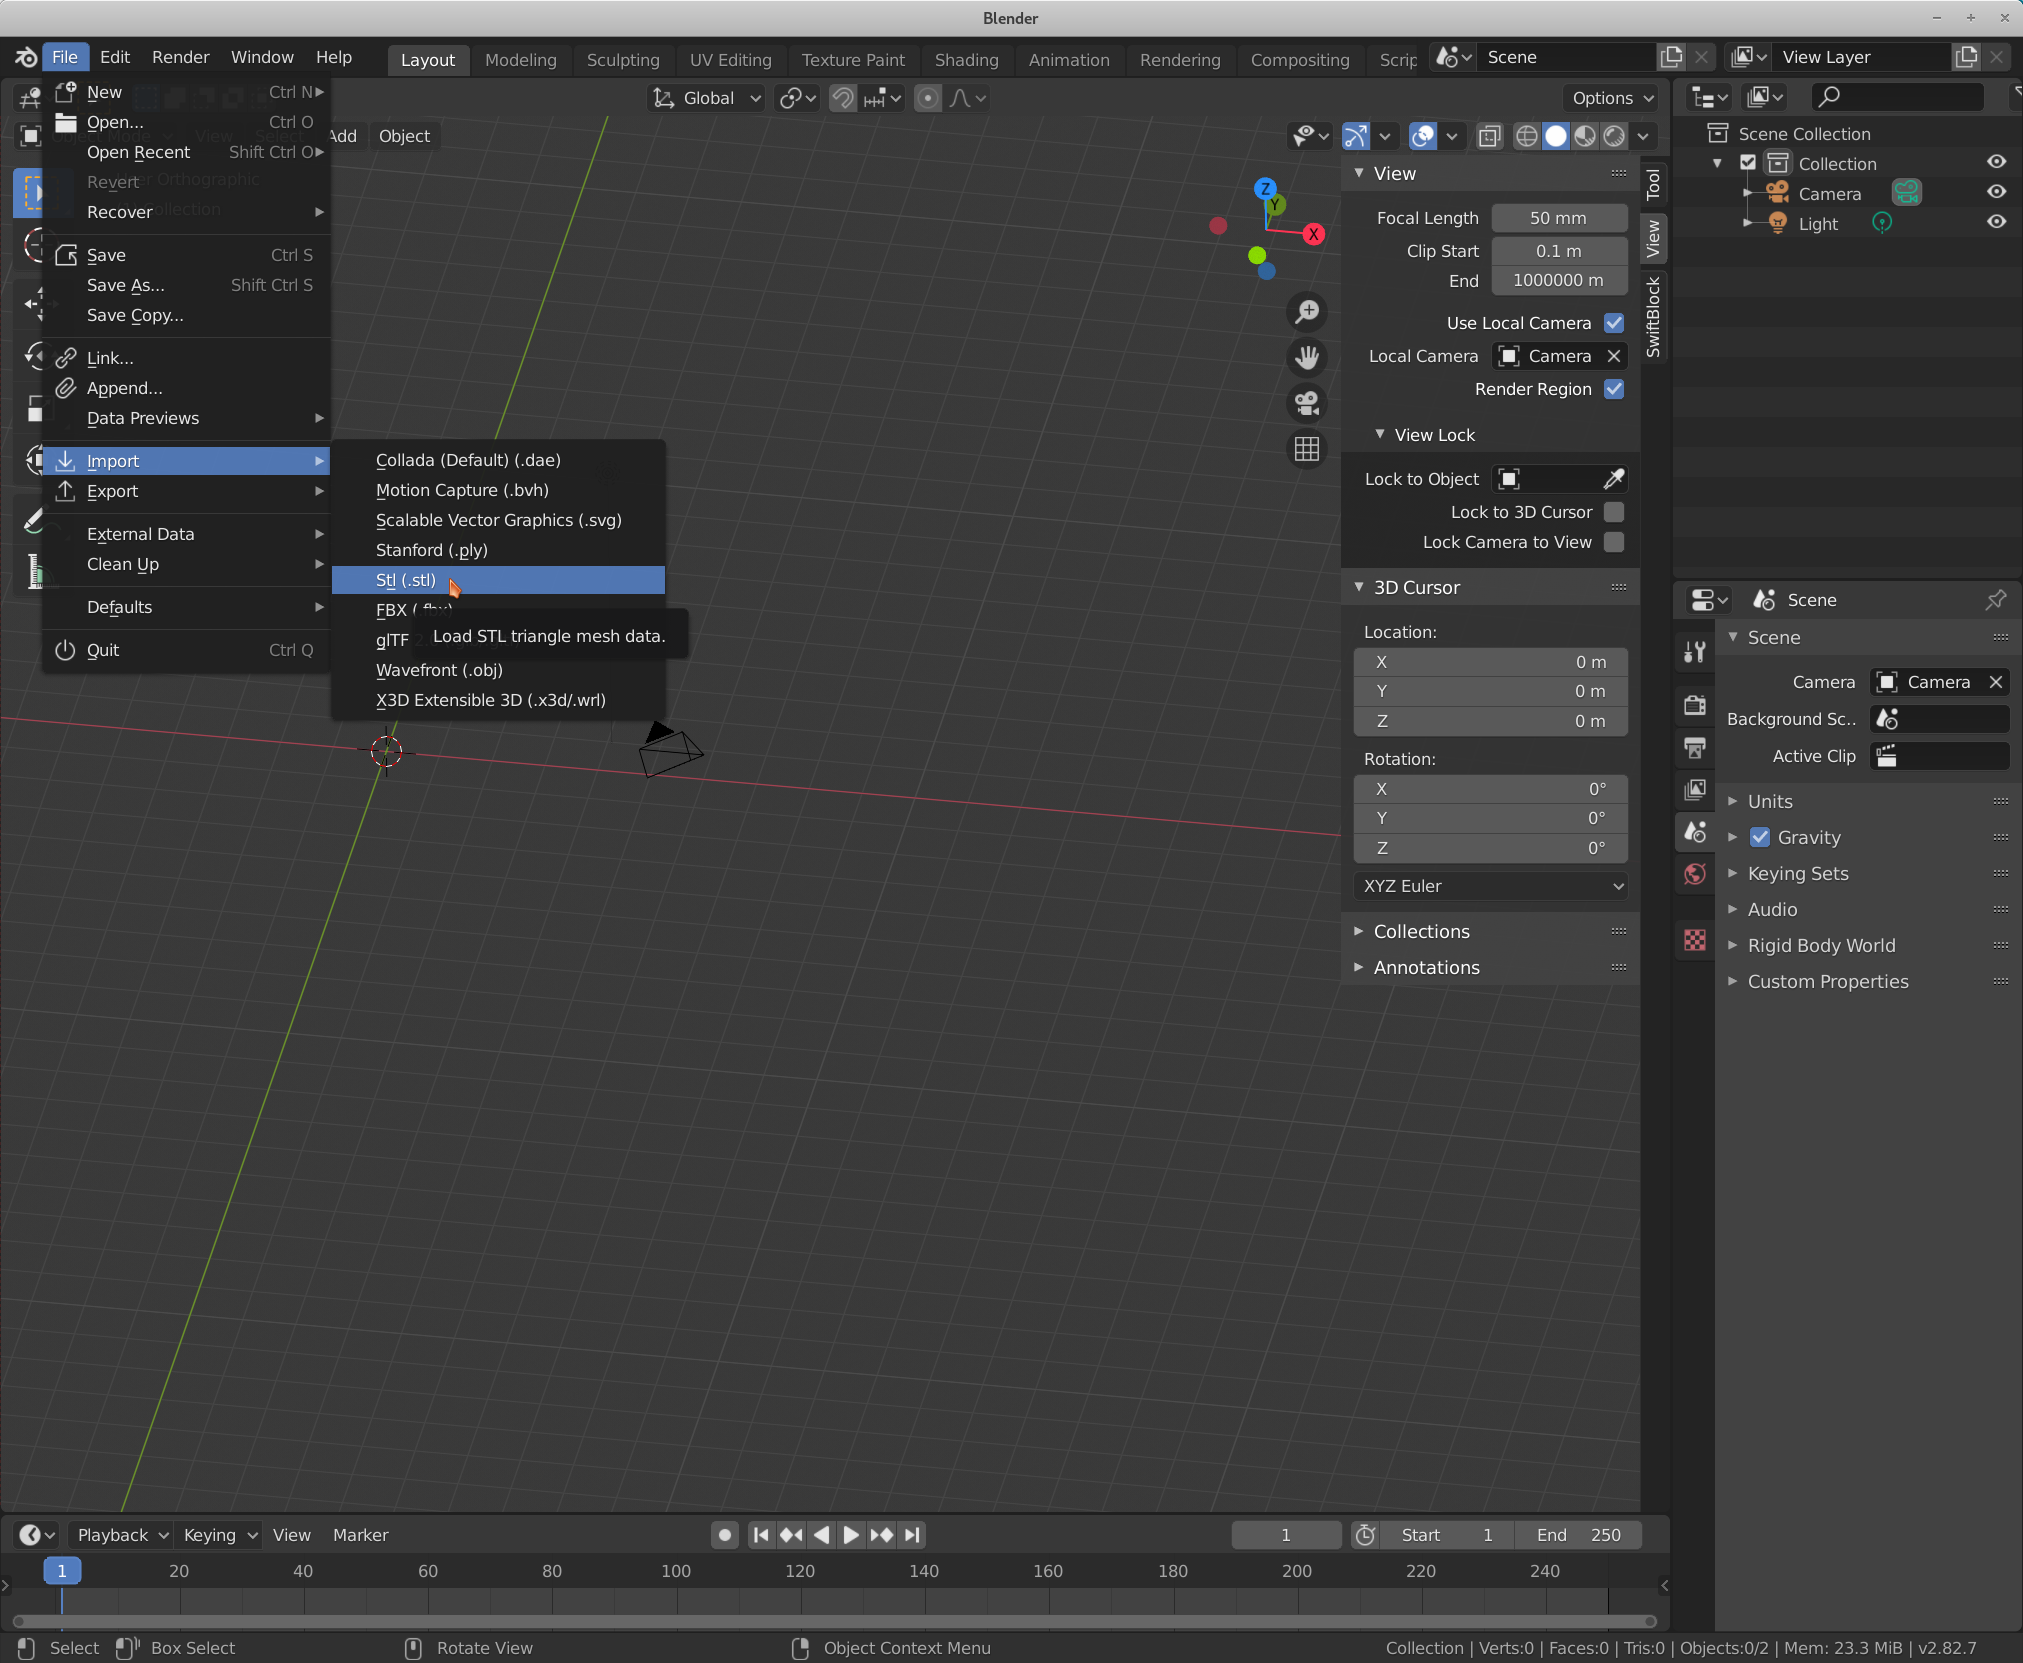
\includegraphics[width=0.75\linewidth]{figs/feature_edges_blender/01_import_stl_1}

\item select the STL file

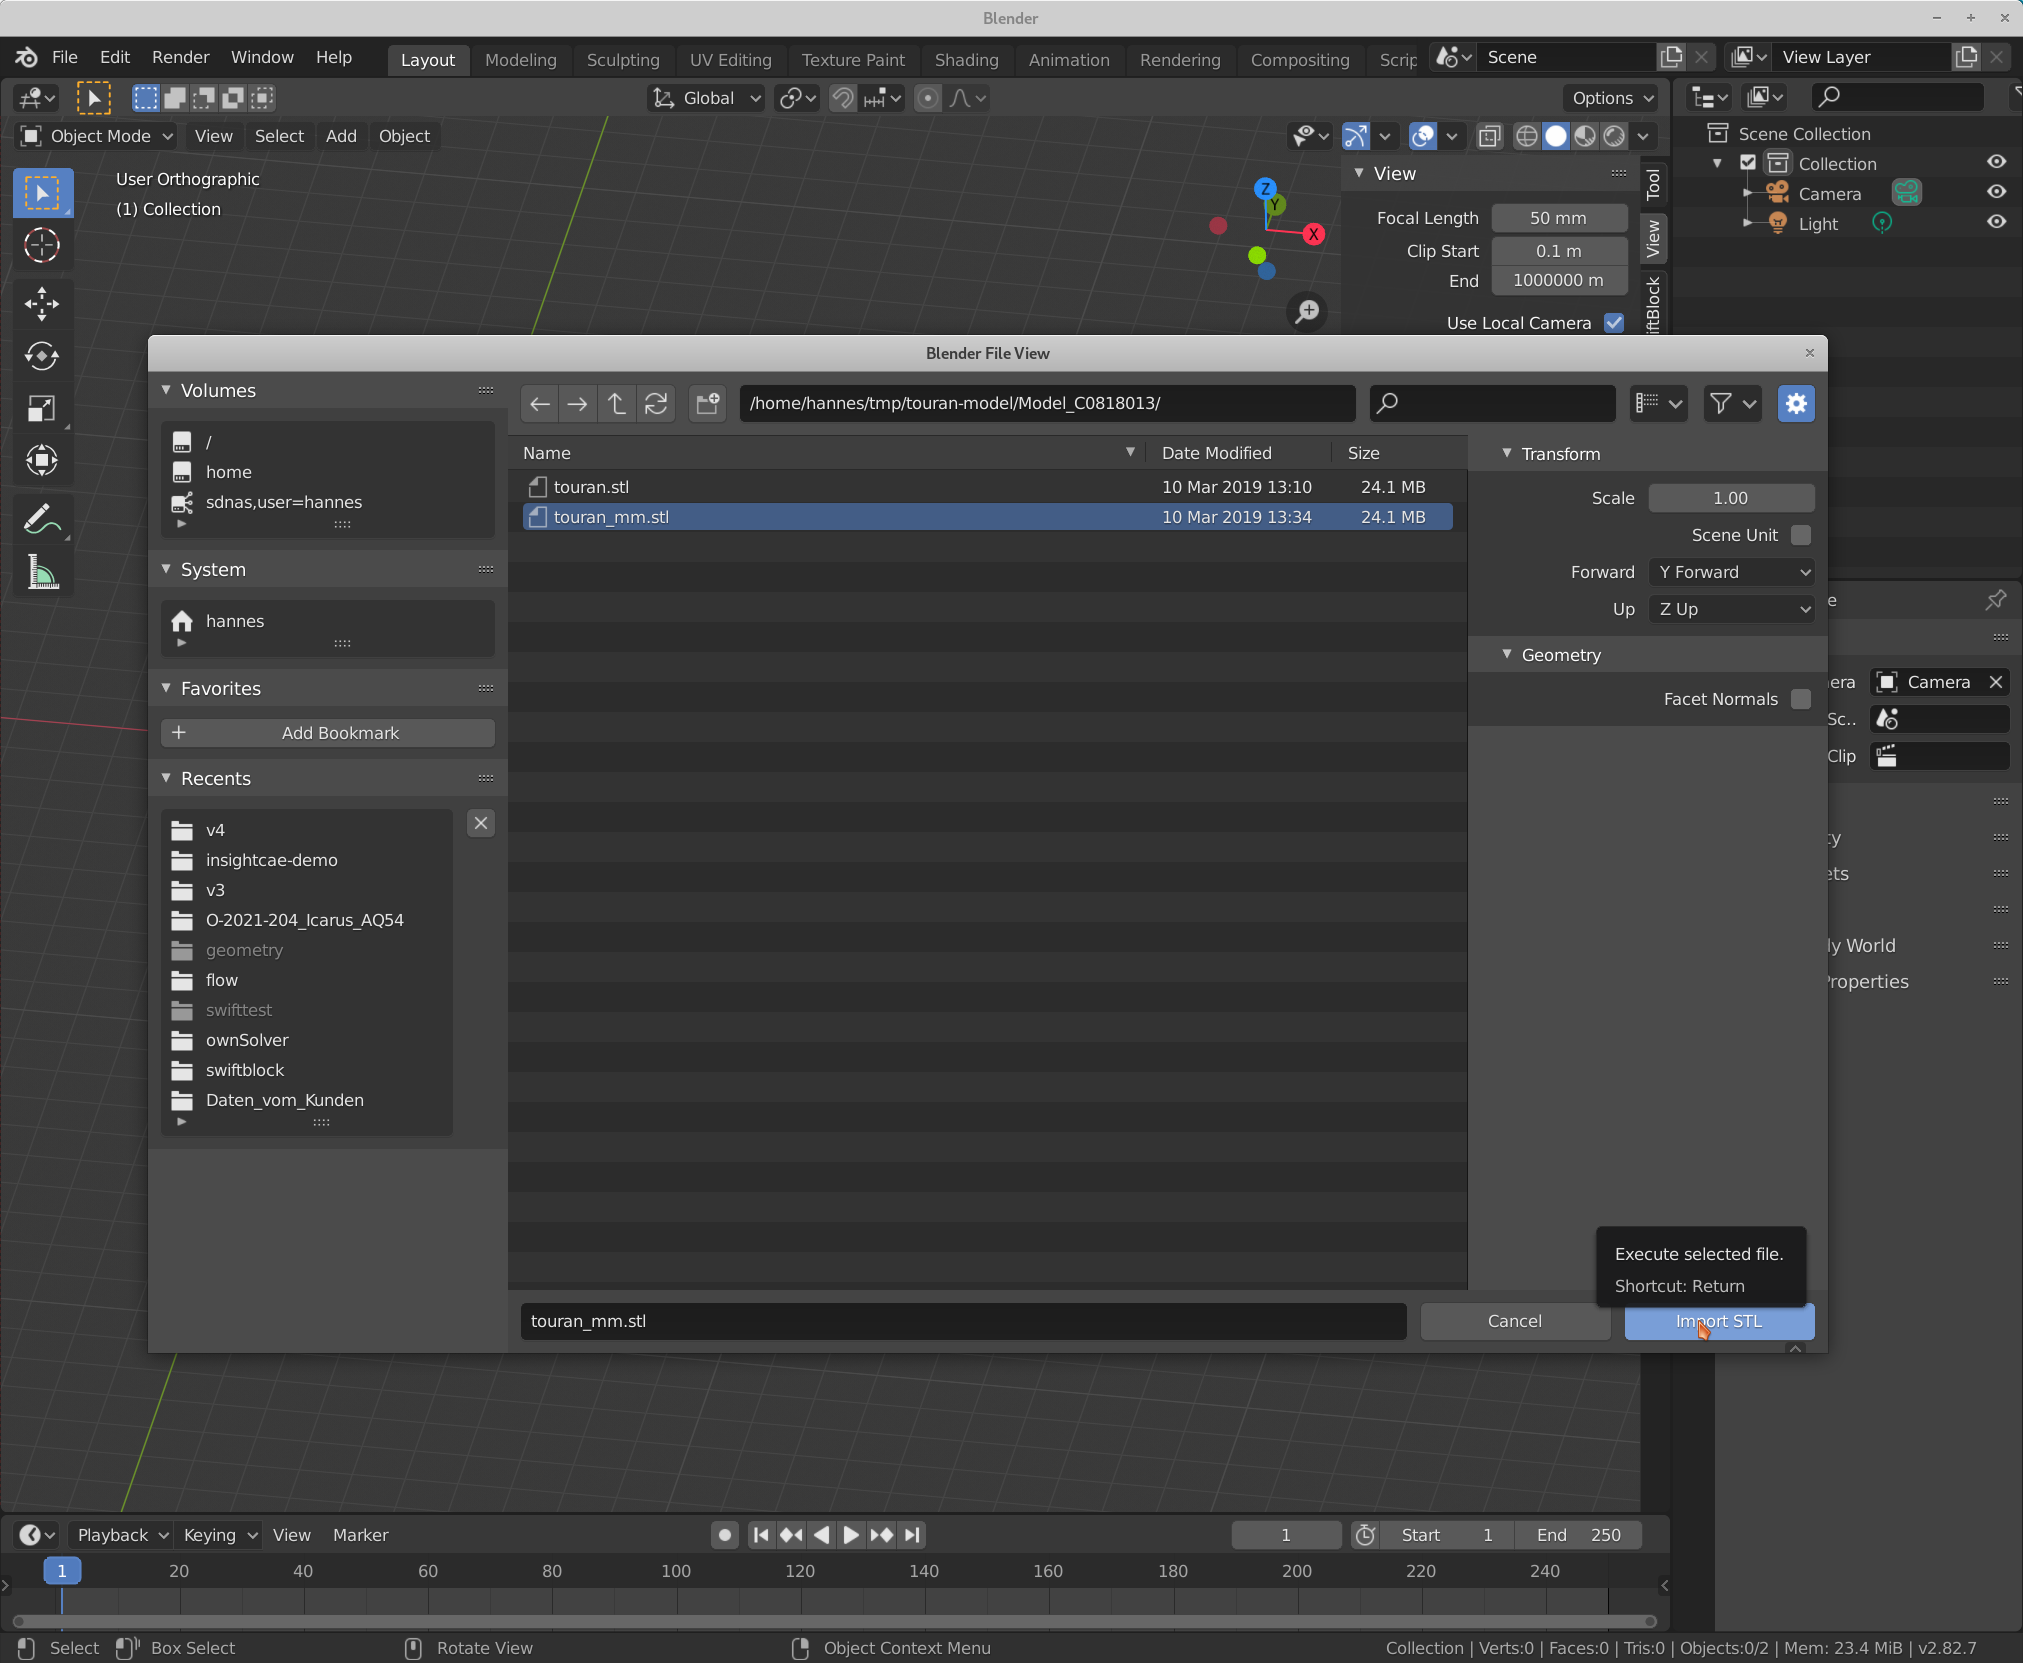
\includegraphics[width=0.75\linewidth]{figs/feature_edges_blender/02_import_stl_2}

\item make sure, the object is selected (orange line around the selected object is displayed)

Objects can be selected by left click them with mouse.

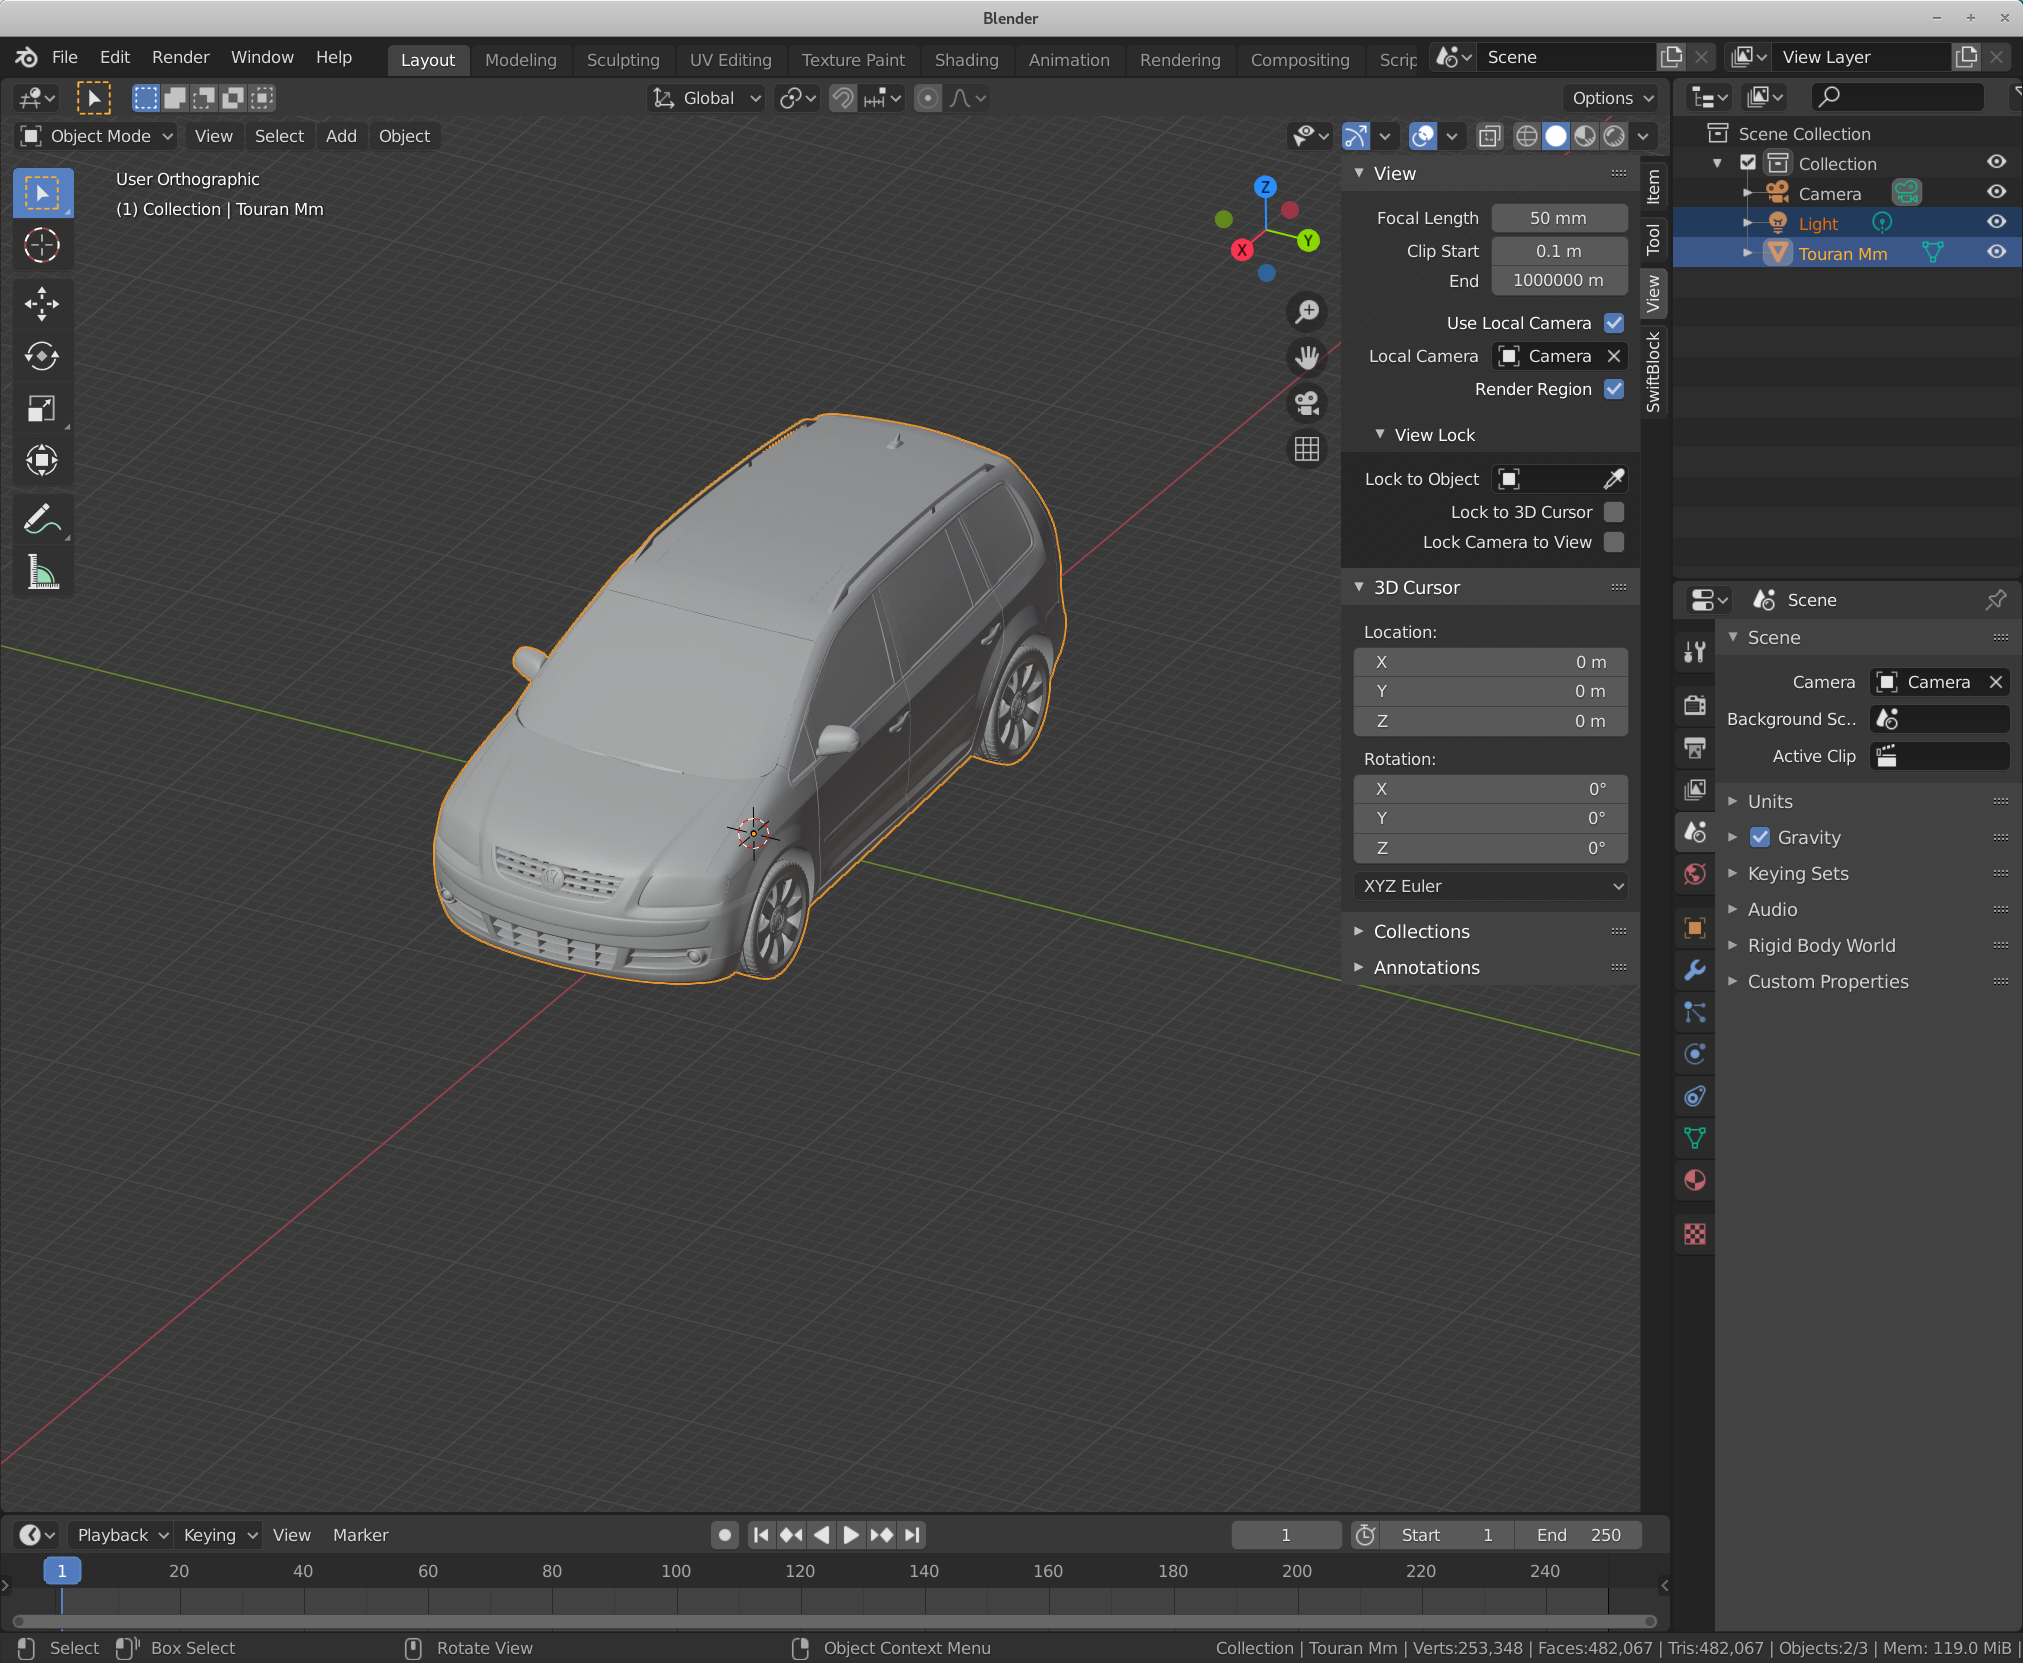
\includegraphics[width=0.75\linewidth]{figs/feature_edges_blender/03_stl_imported}

\item switch to "Edit Mode", either by pressing the "Tab" key or by selecting the mode in the combo box in the upper left corner.

Next, switch to edge selection mode (second button right from the edit mode combo box)

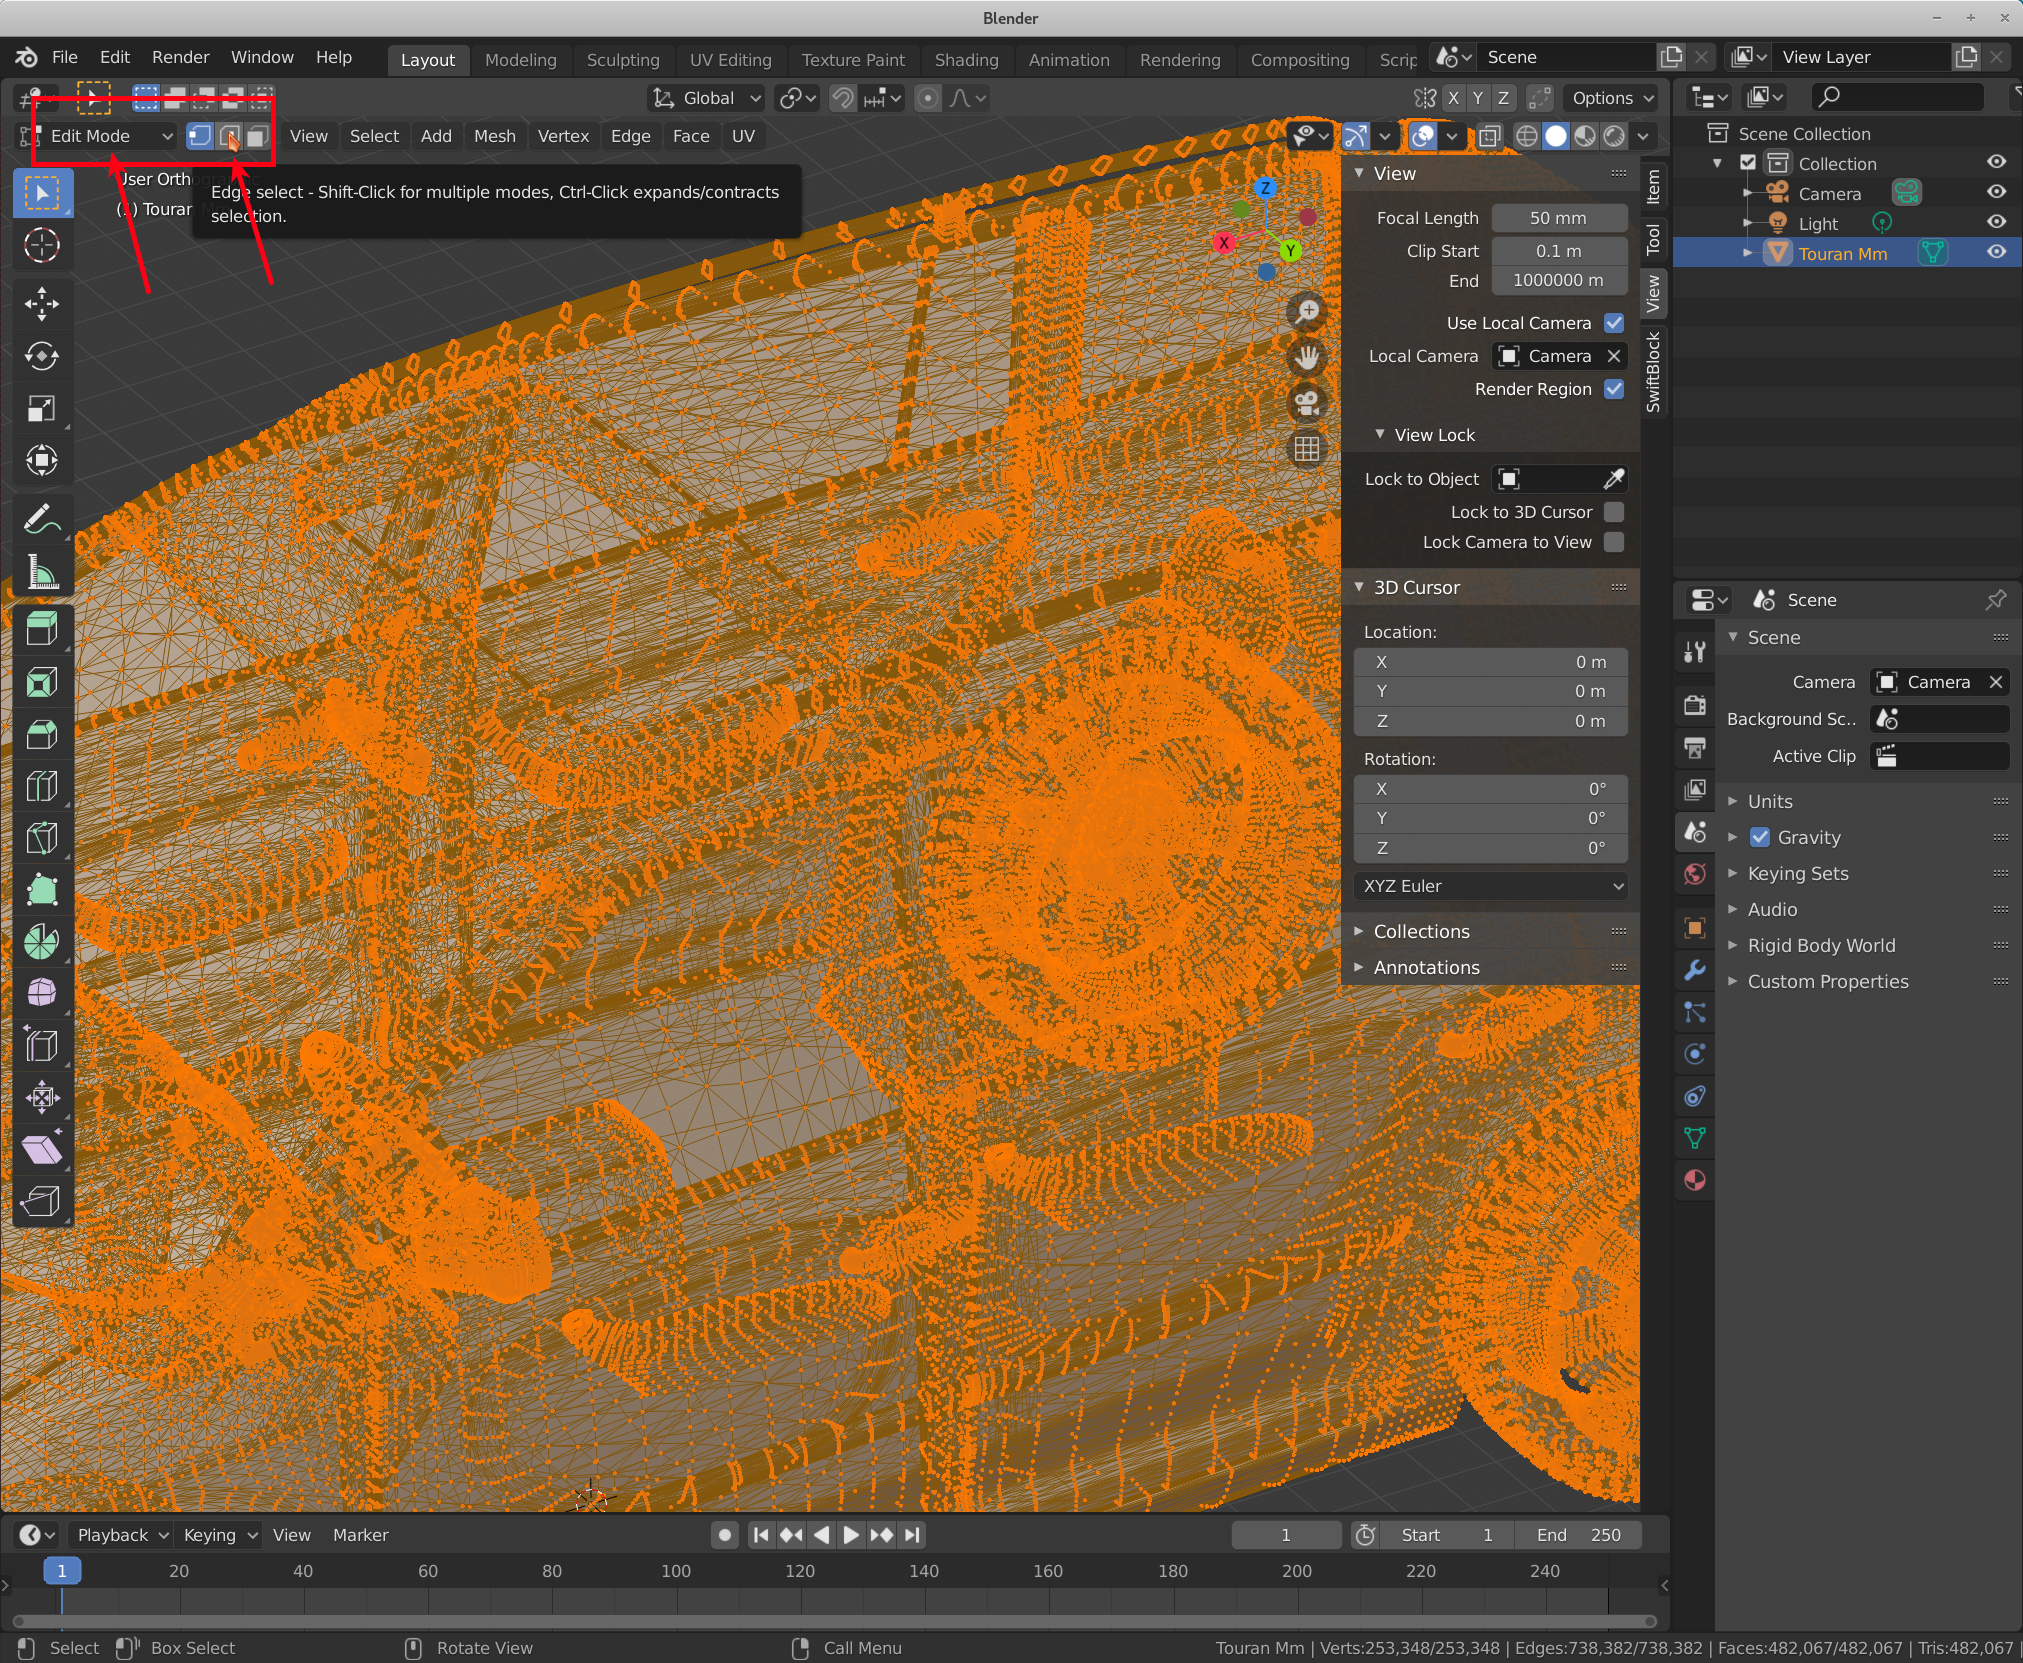
\includegraphics[width=0.75\linewidth]{figs/feature_edges_blender/04_edit_mode}

In this example, we want to select a line (chain of edges) along the left roof rail.

\item zoom into the location of the beginning of the line
\label{pt:begin_sel}

select the first edge with a left click on it.

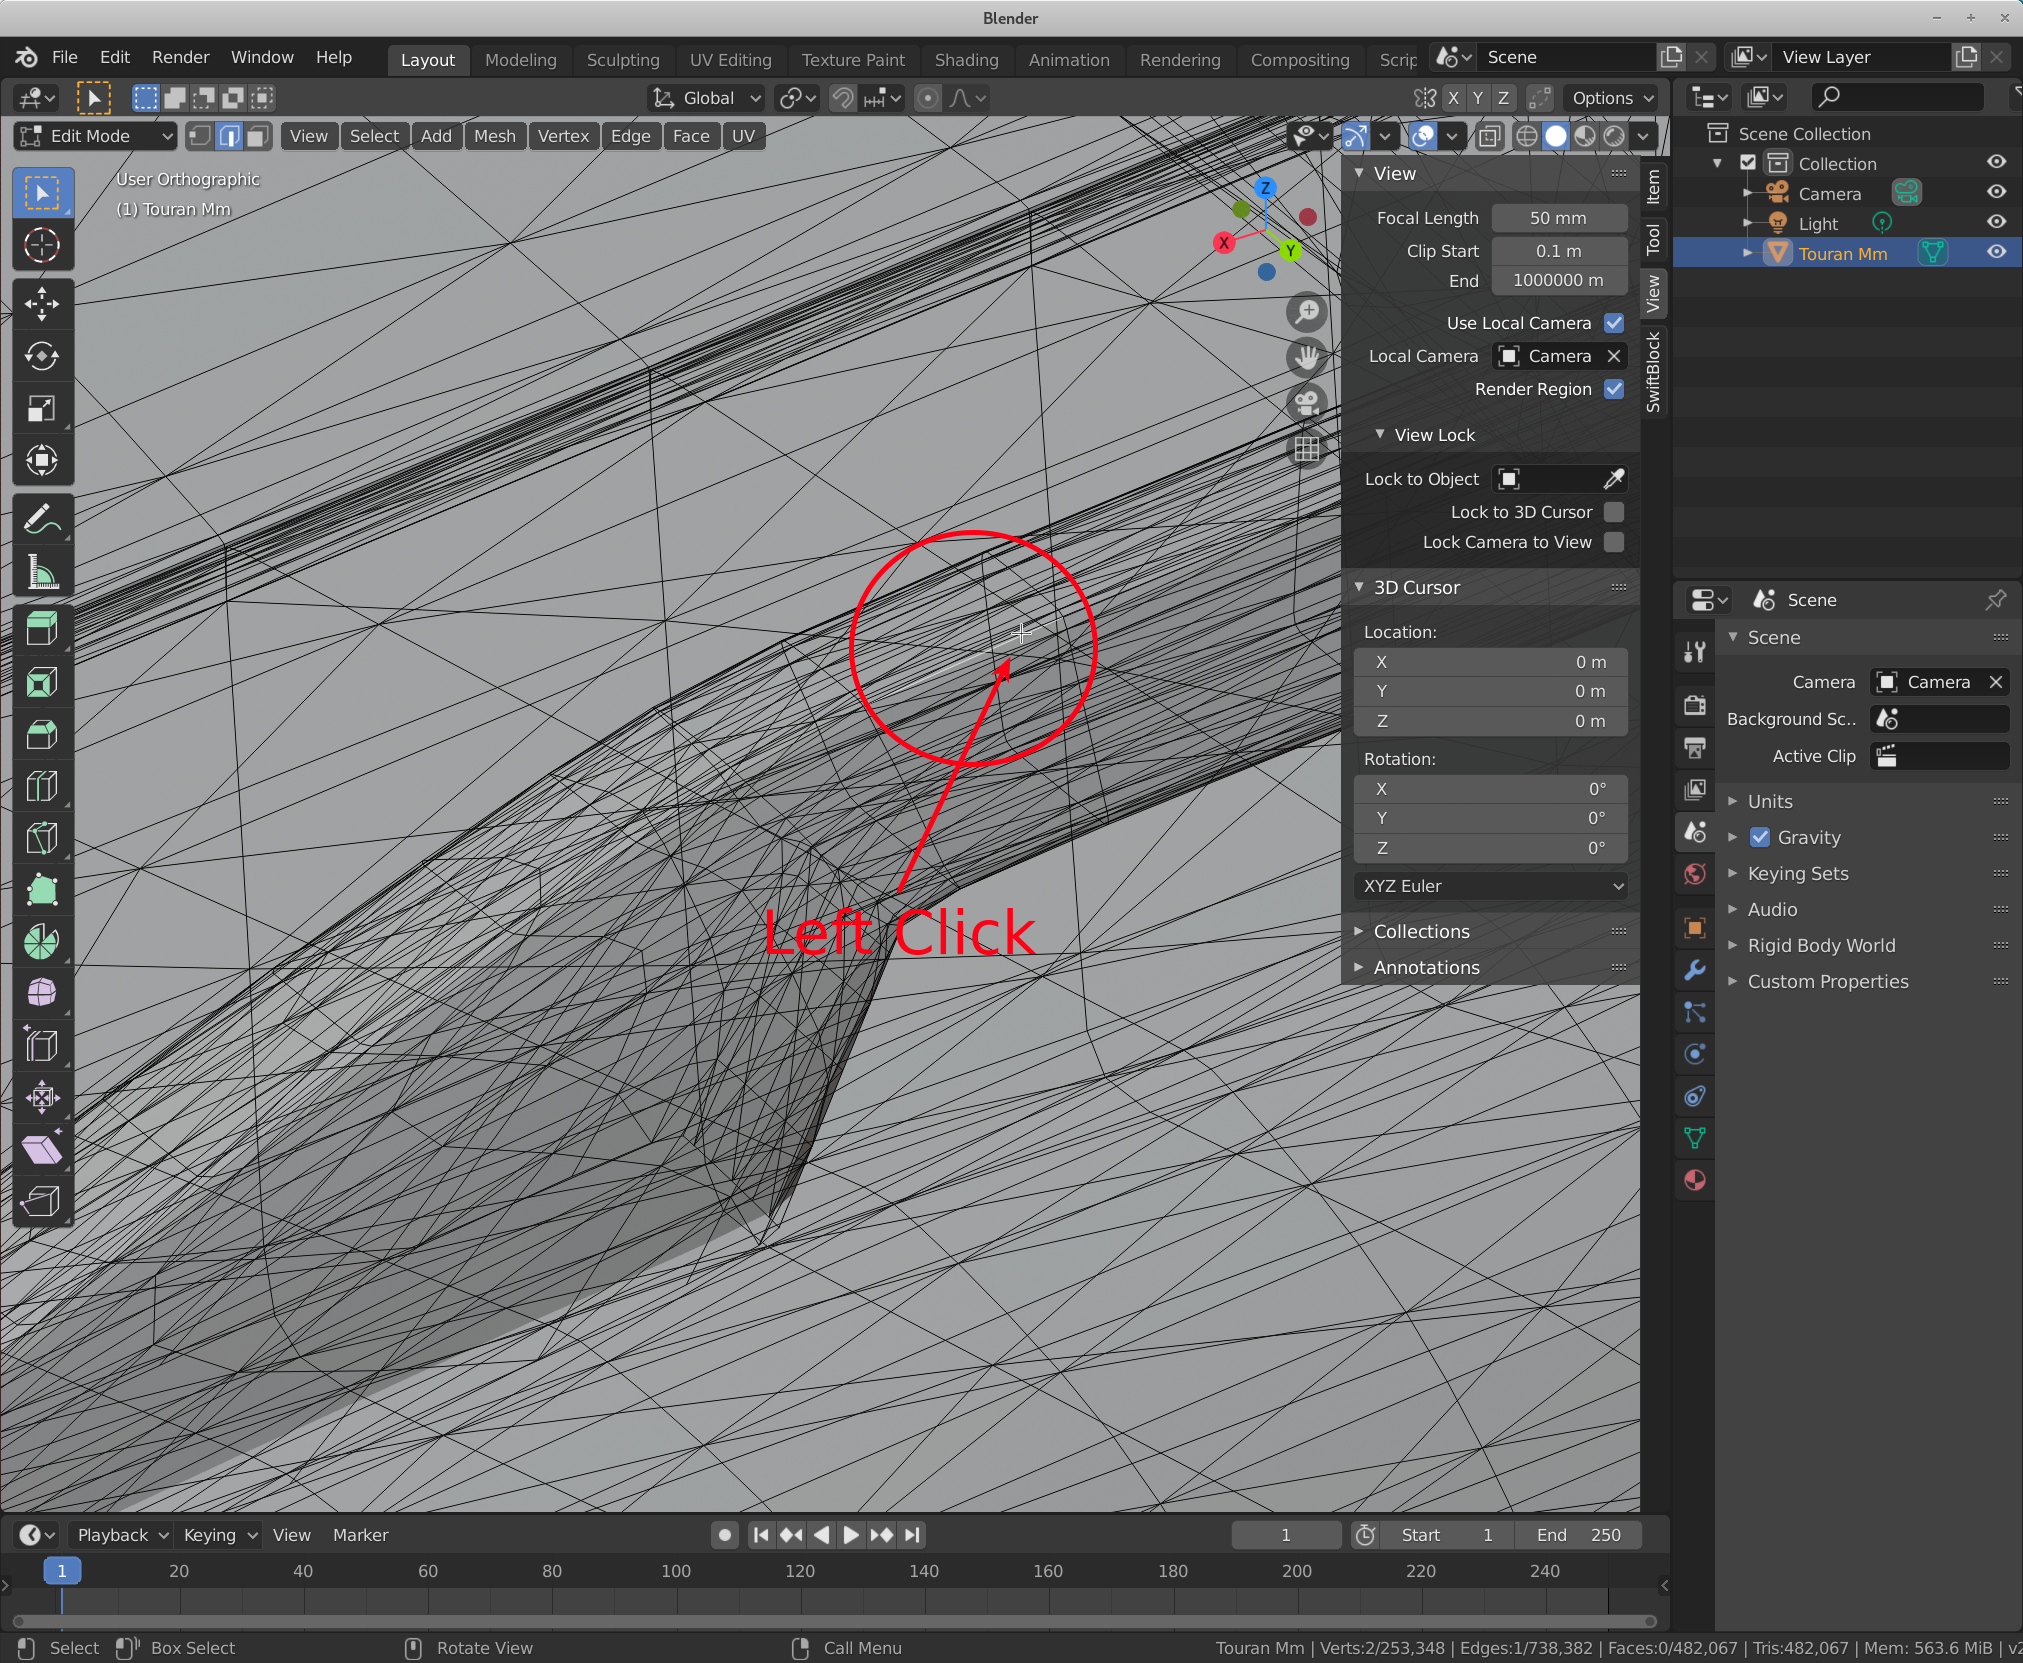
\includegraphics[width=0.75\linewidth]{figs/feature_edges_blender/05_select_first_edge}

\item select another edge on the feature line: zoom to the next location and press Ctrl + Left click

The shortest path from the last selected edge and the current clicked edge will be added to the selection.
To select edges as precise as possible, it might be required to click a number of intermediate locations.
If a mistake is made, the last step can be undone by typing Ctrl+Z.

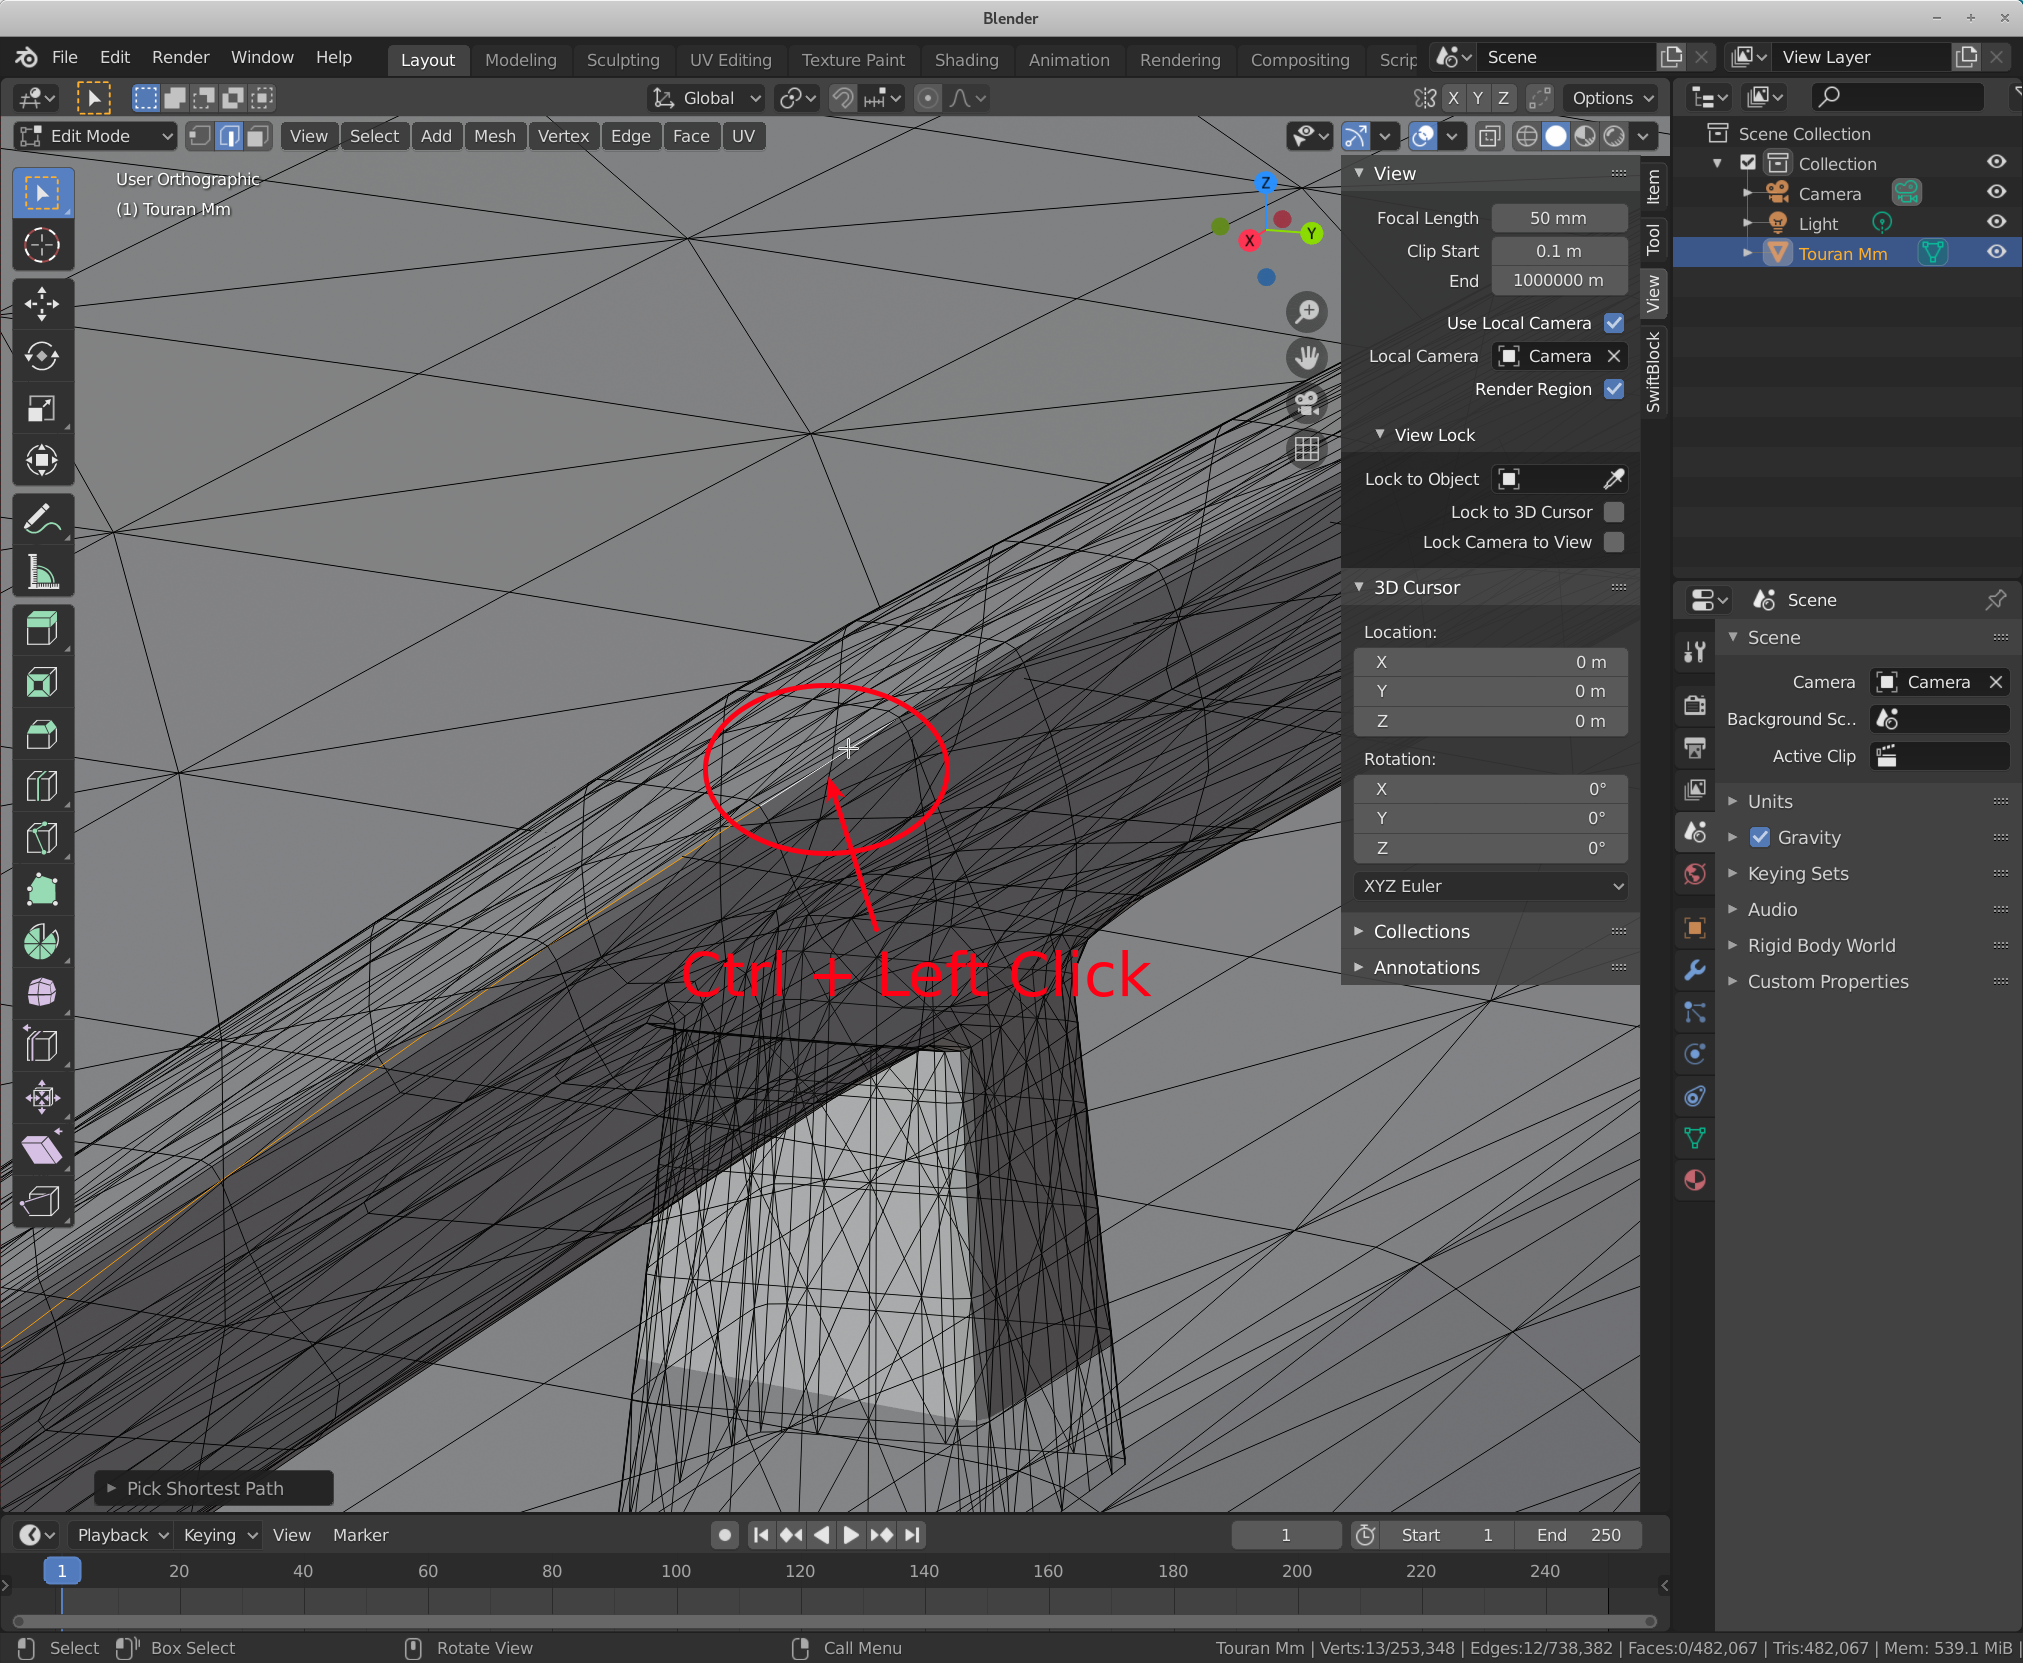
\includegraphics[width=0.75\linewidth]{figs/feature_edges_blender/06_select_second_edge}

\item repeat the last step until the end of the feature line is reached.

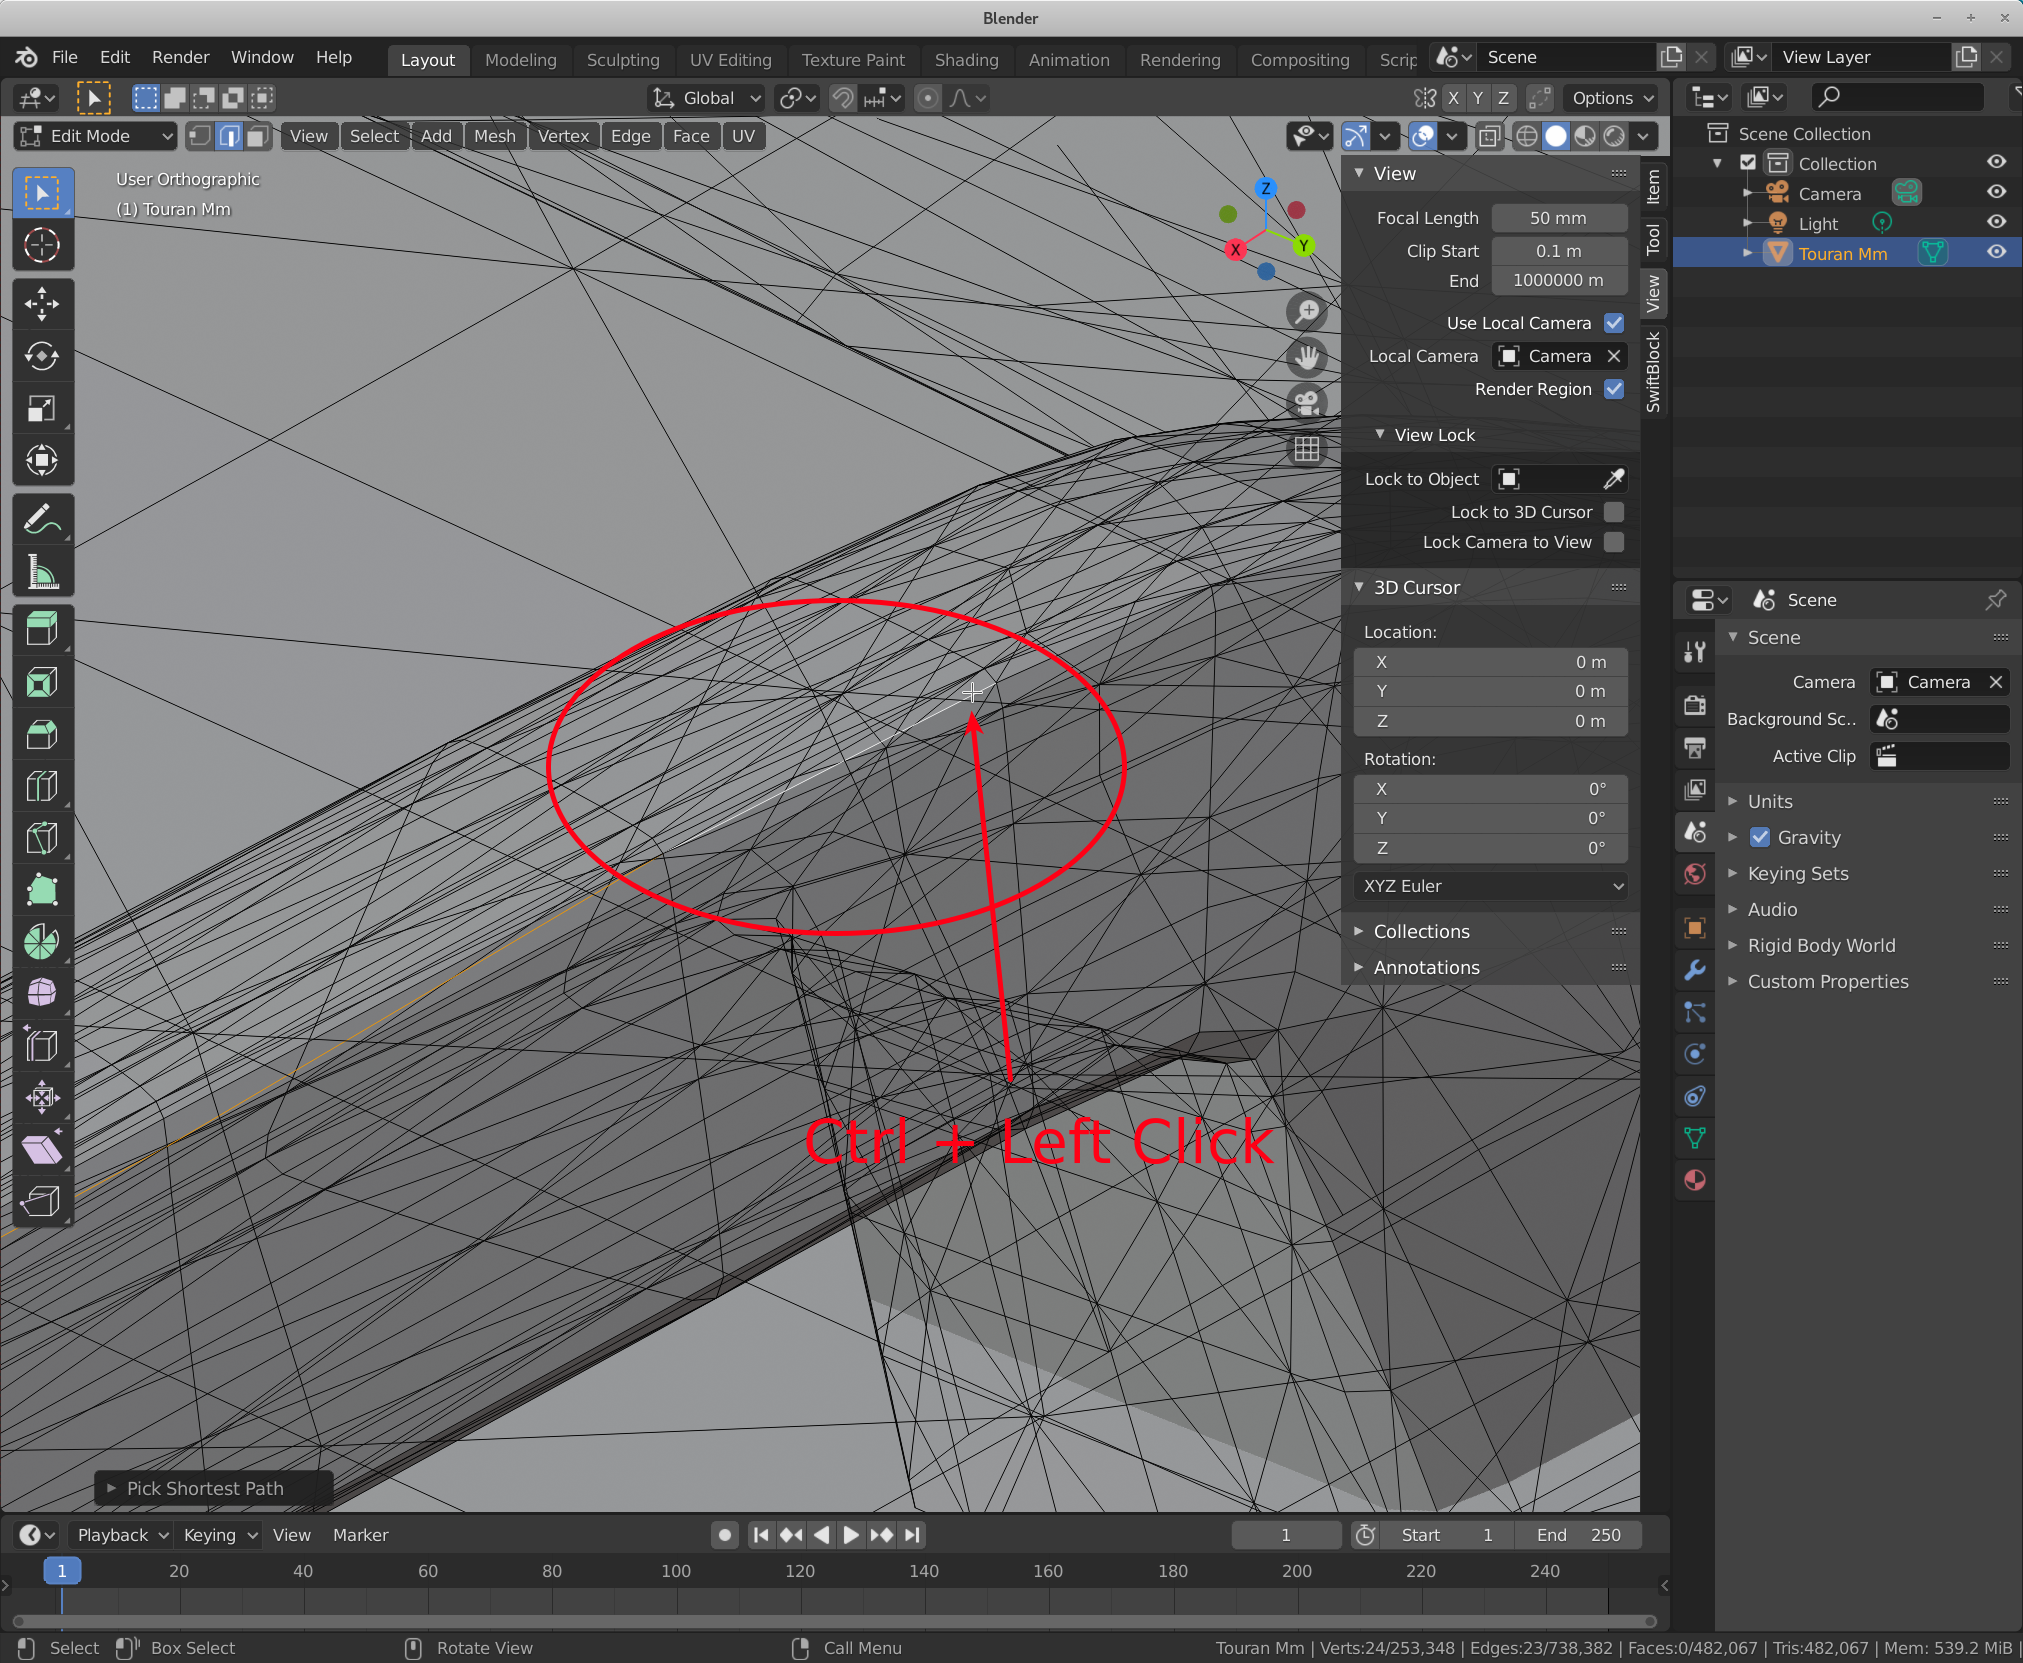
\includegraphics[width=0.75\linewidth]{figs/feature_edges_blender/07_select_last_edge}

\item next create a new object from the selected edges by typing the key "P".

Then select "Selection" to create the new part from the current selection.

Once the selection is split off, another chain of edges can be selected by repeating the steps from \ref{pt:begin_sel}.

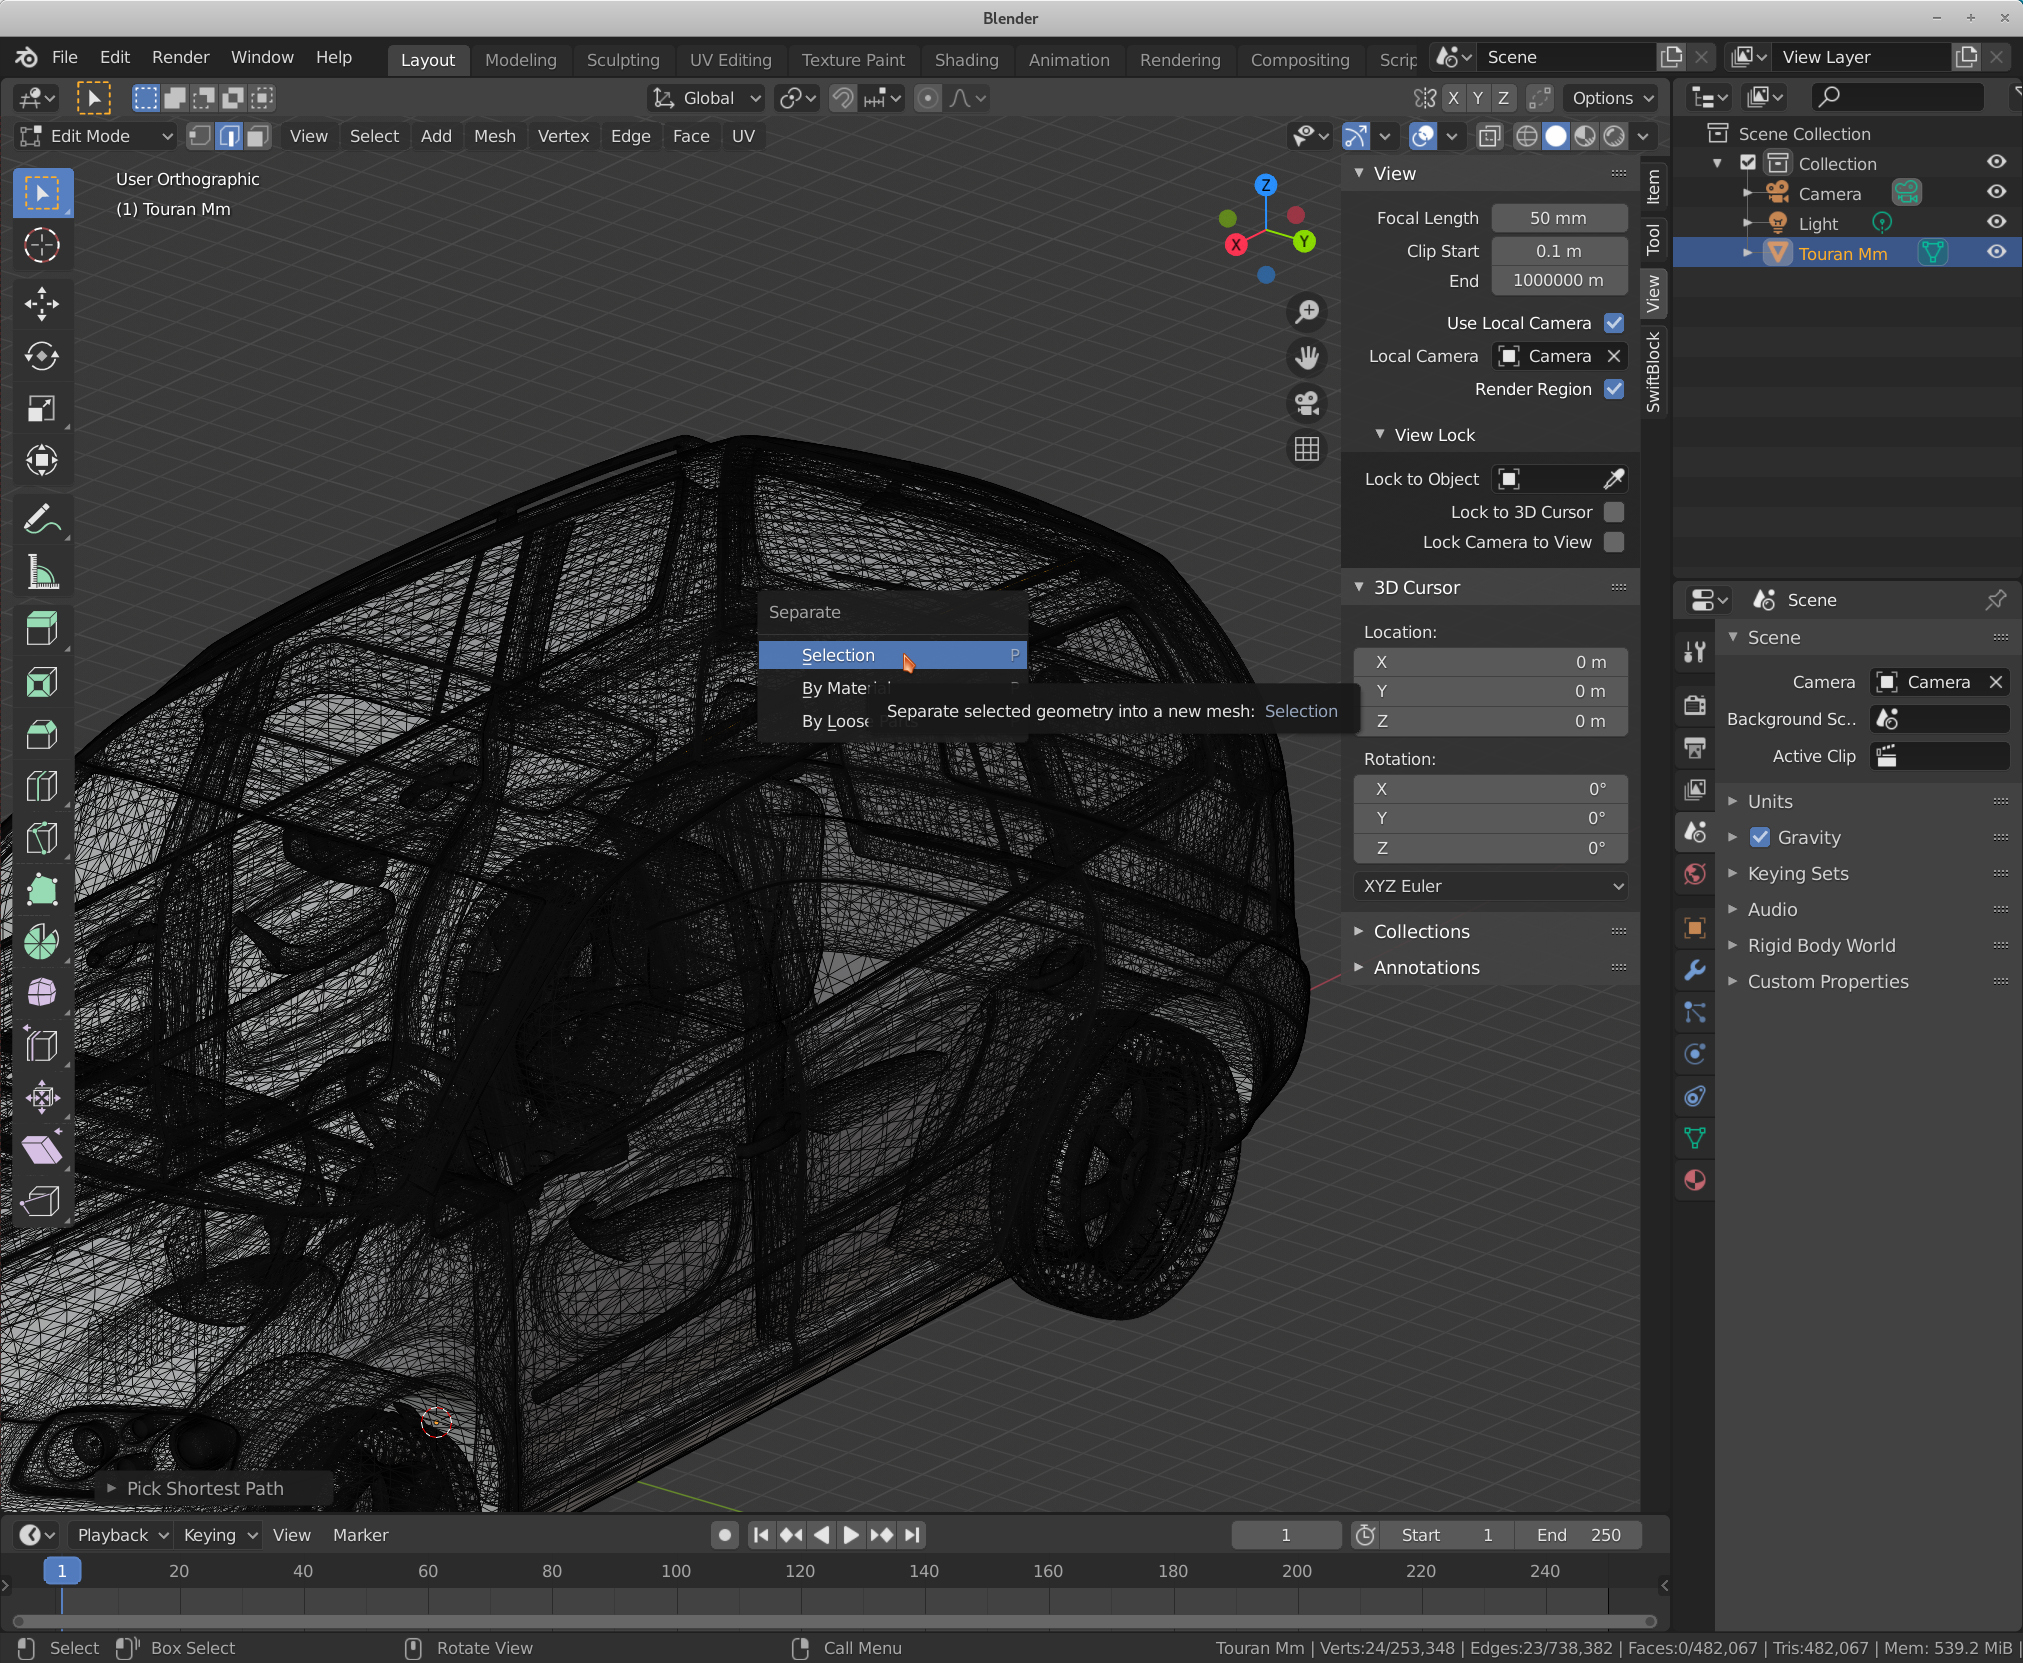
\includegraphics[width=0.75\linewidth]{figs/feature_edges_blender/08_export_selection}

\item switch back to "Object Mode"

either by pressing the Tab key or by selecting "Object Mode" in the combo box in the upper left corner.

When multiple lines had been split into multiple new objects, these should be joined into a single one.
To do so, select the objects in the object browser (upper right), then type "Ctrl+J".

Note: the mouse should be over the 3D viewport for Blender to accept the keyboard shortcut.

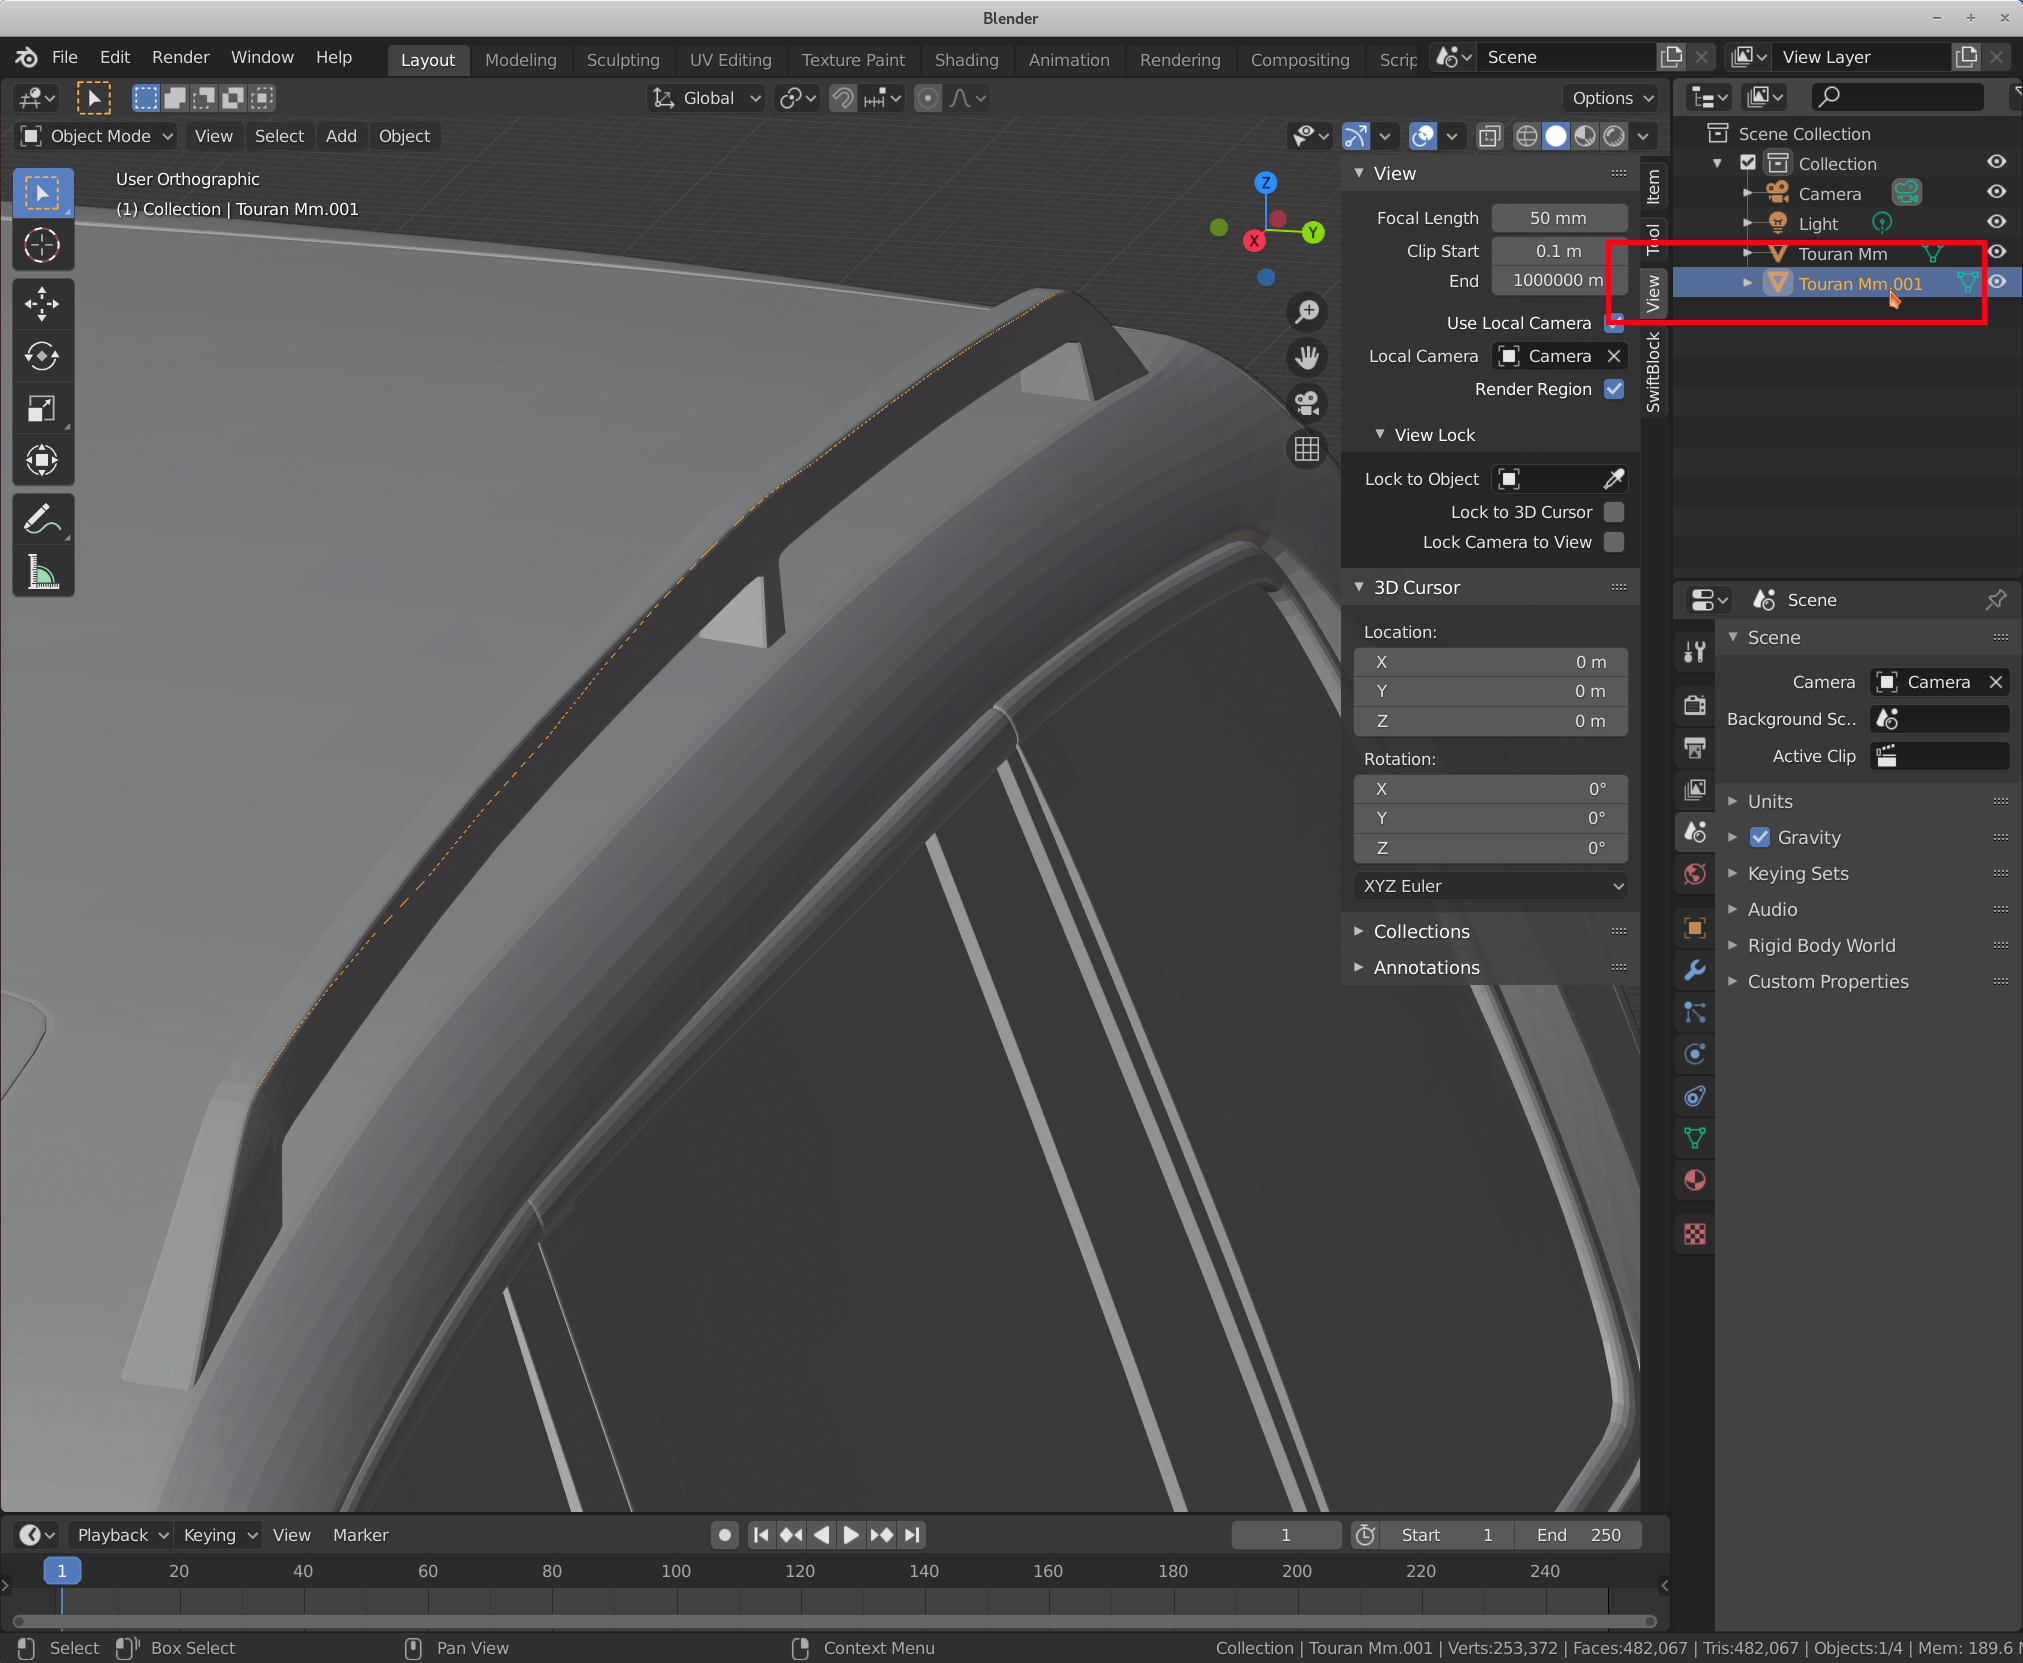
\includegraphics[width=0.75\linewidth]{figs/feature_edges_blender/09_view_result}

\item export the edges into an OBJ file.

Select the object in the object browser with a left click.

Then open the menu \menu{File>Export>Wavefront (*.obj)}.

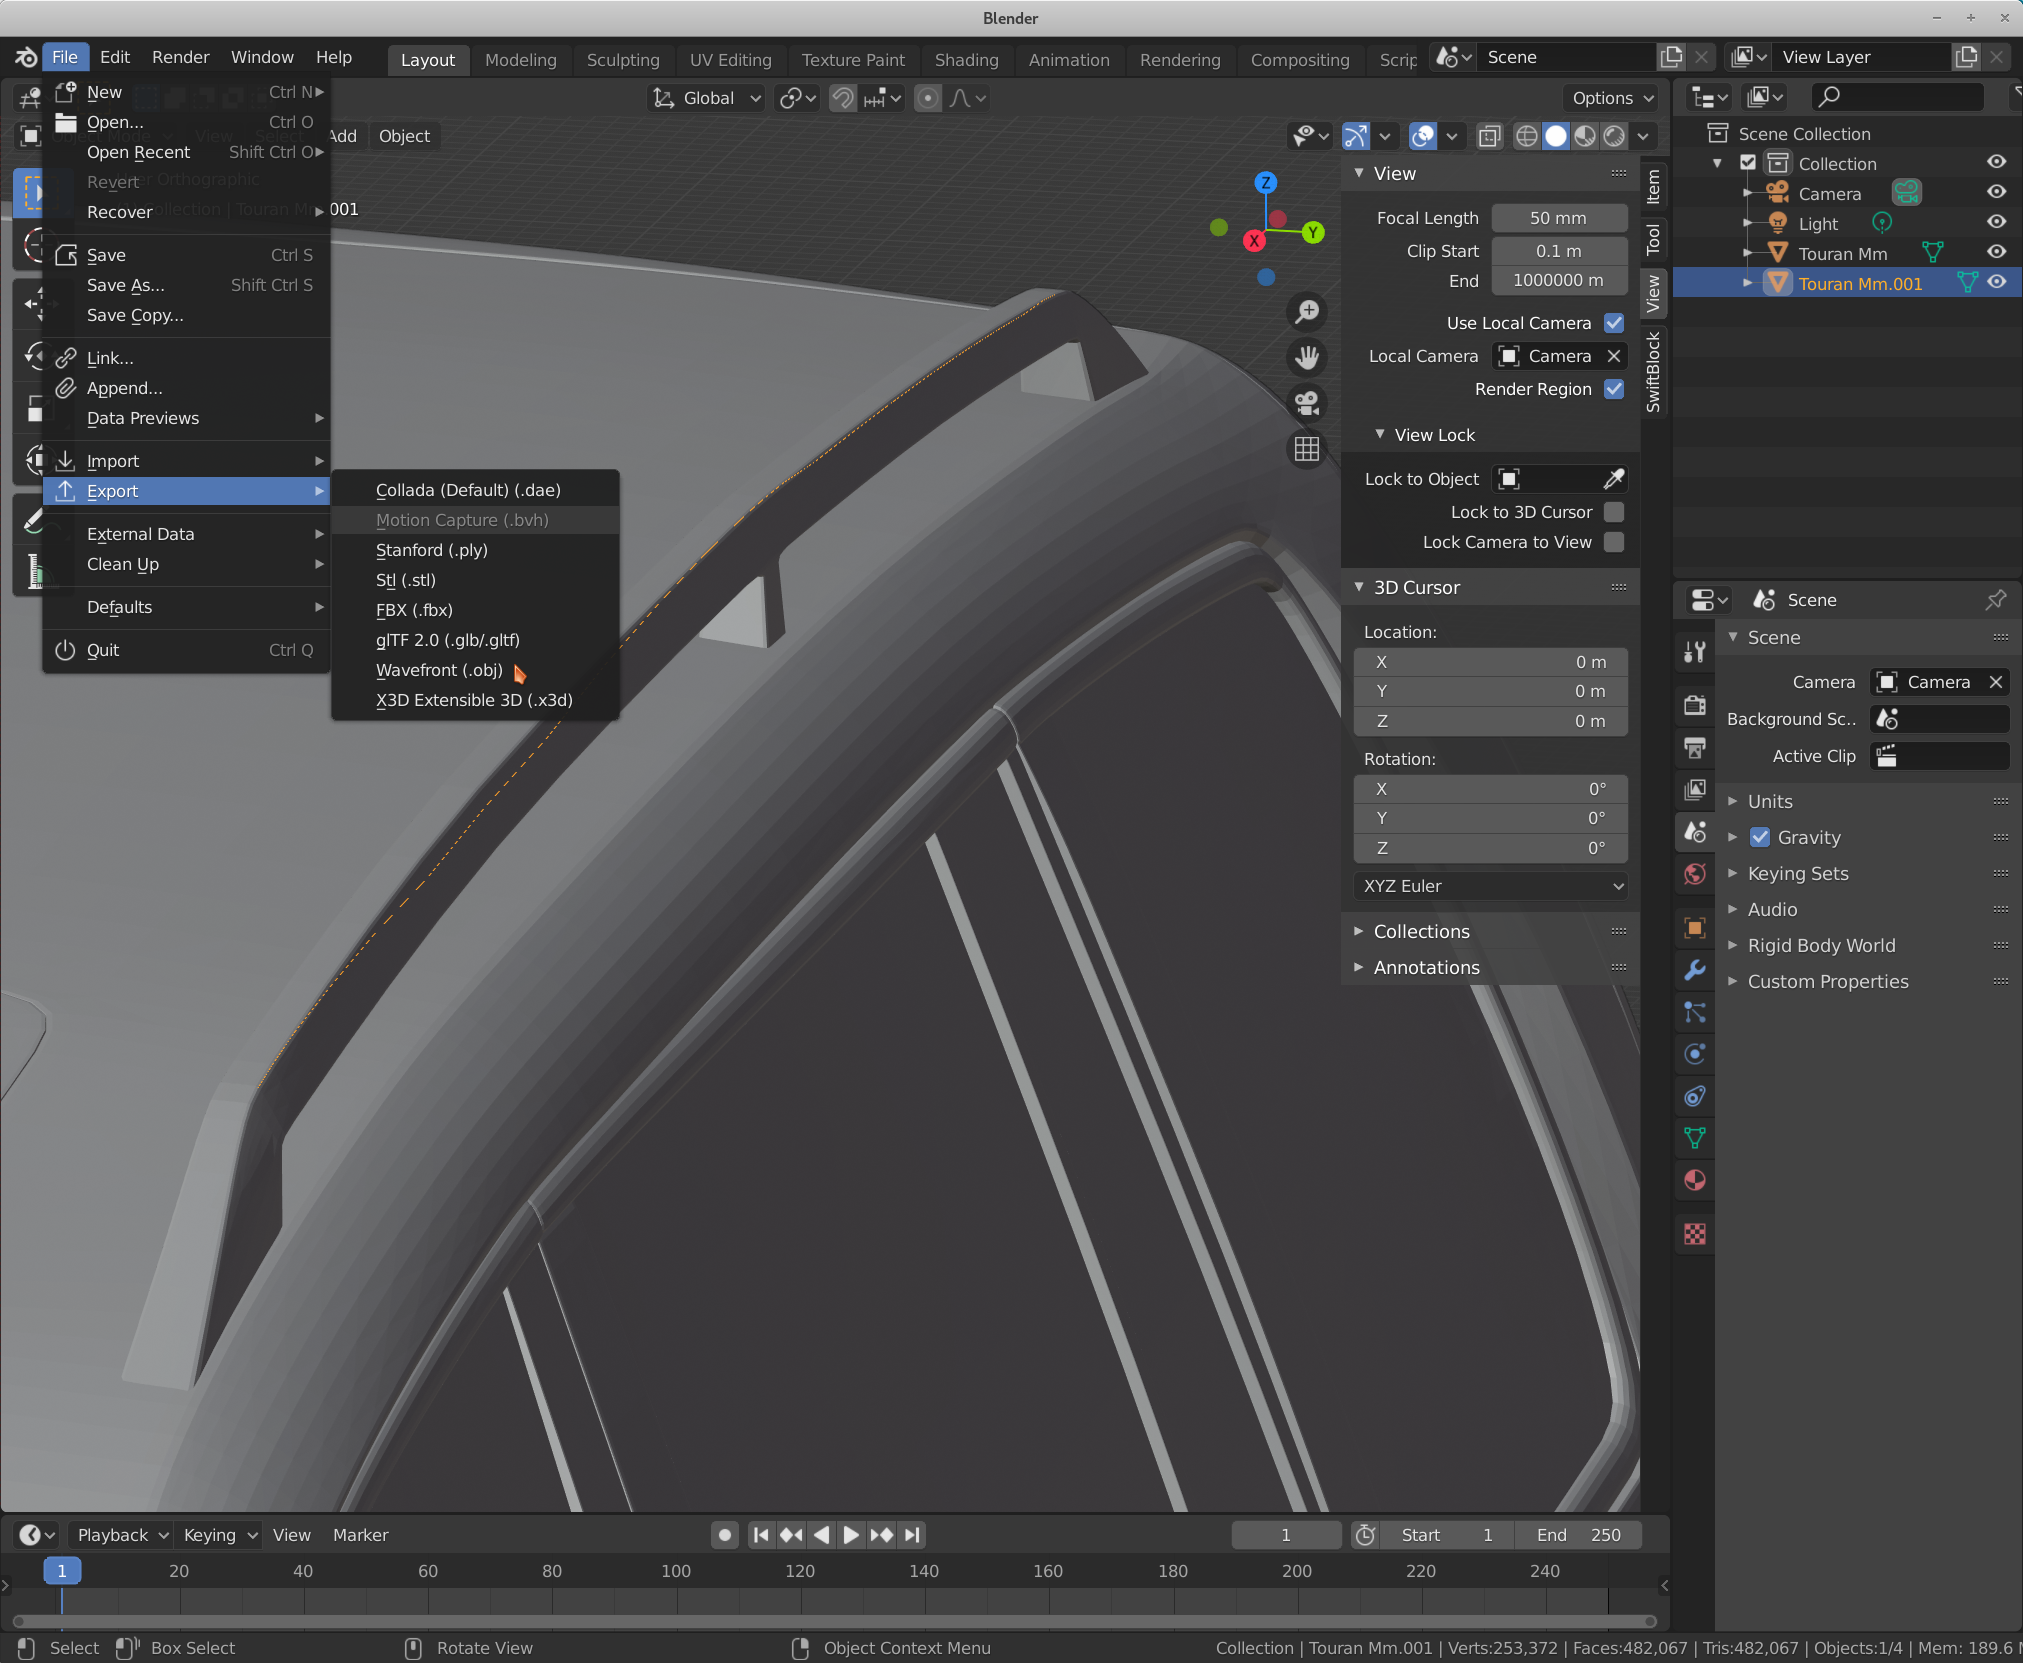
\includegraphics[width=0.75\linewidth]{figs/feature_edges_blender/10_export_obj}

\item check the export settings. Make sure, the following is set:

\begin{itemize}
\item "Selection only" is checked

(Otherwise also the surface will be included in the exported file)
\item In "Transform", "Forward" is set to "Y Forward"

(Otherwise the geometry will be wrongly oriented after export)
\end{itemize}


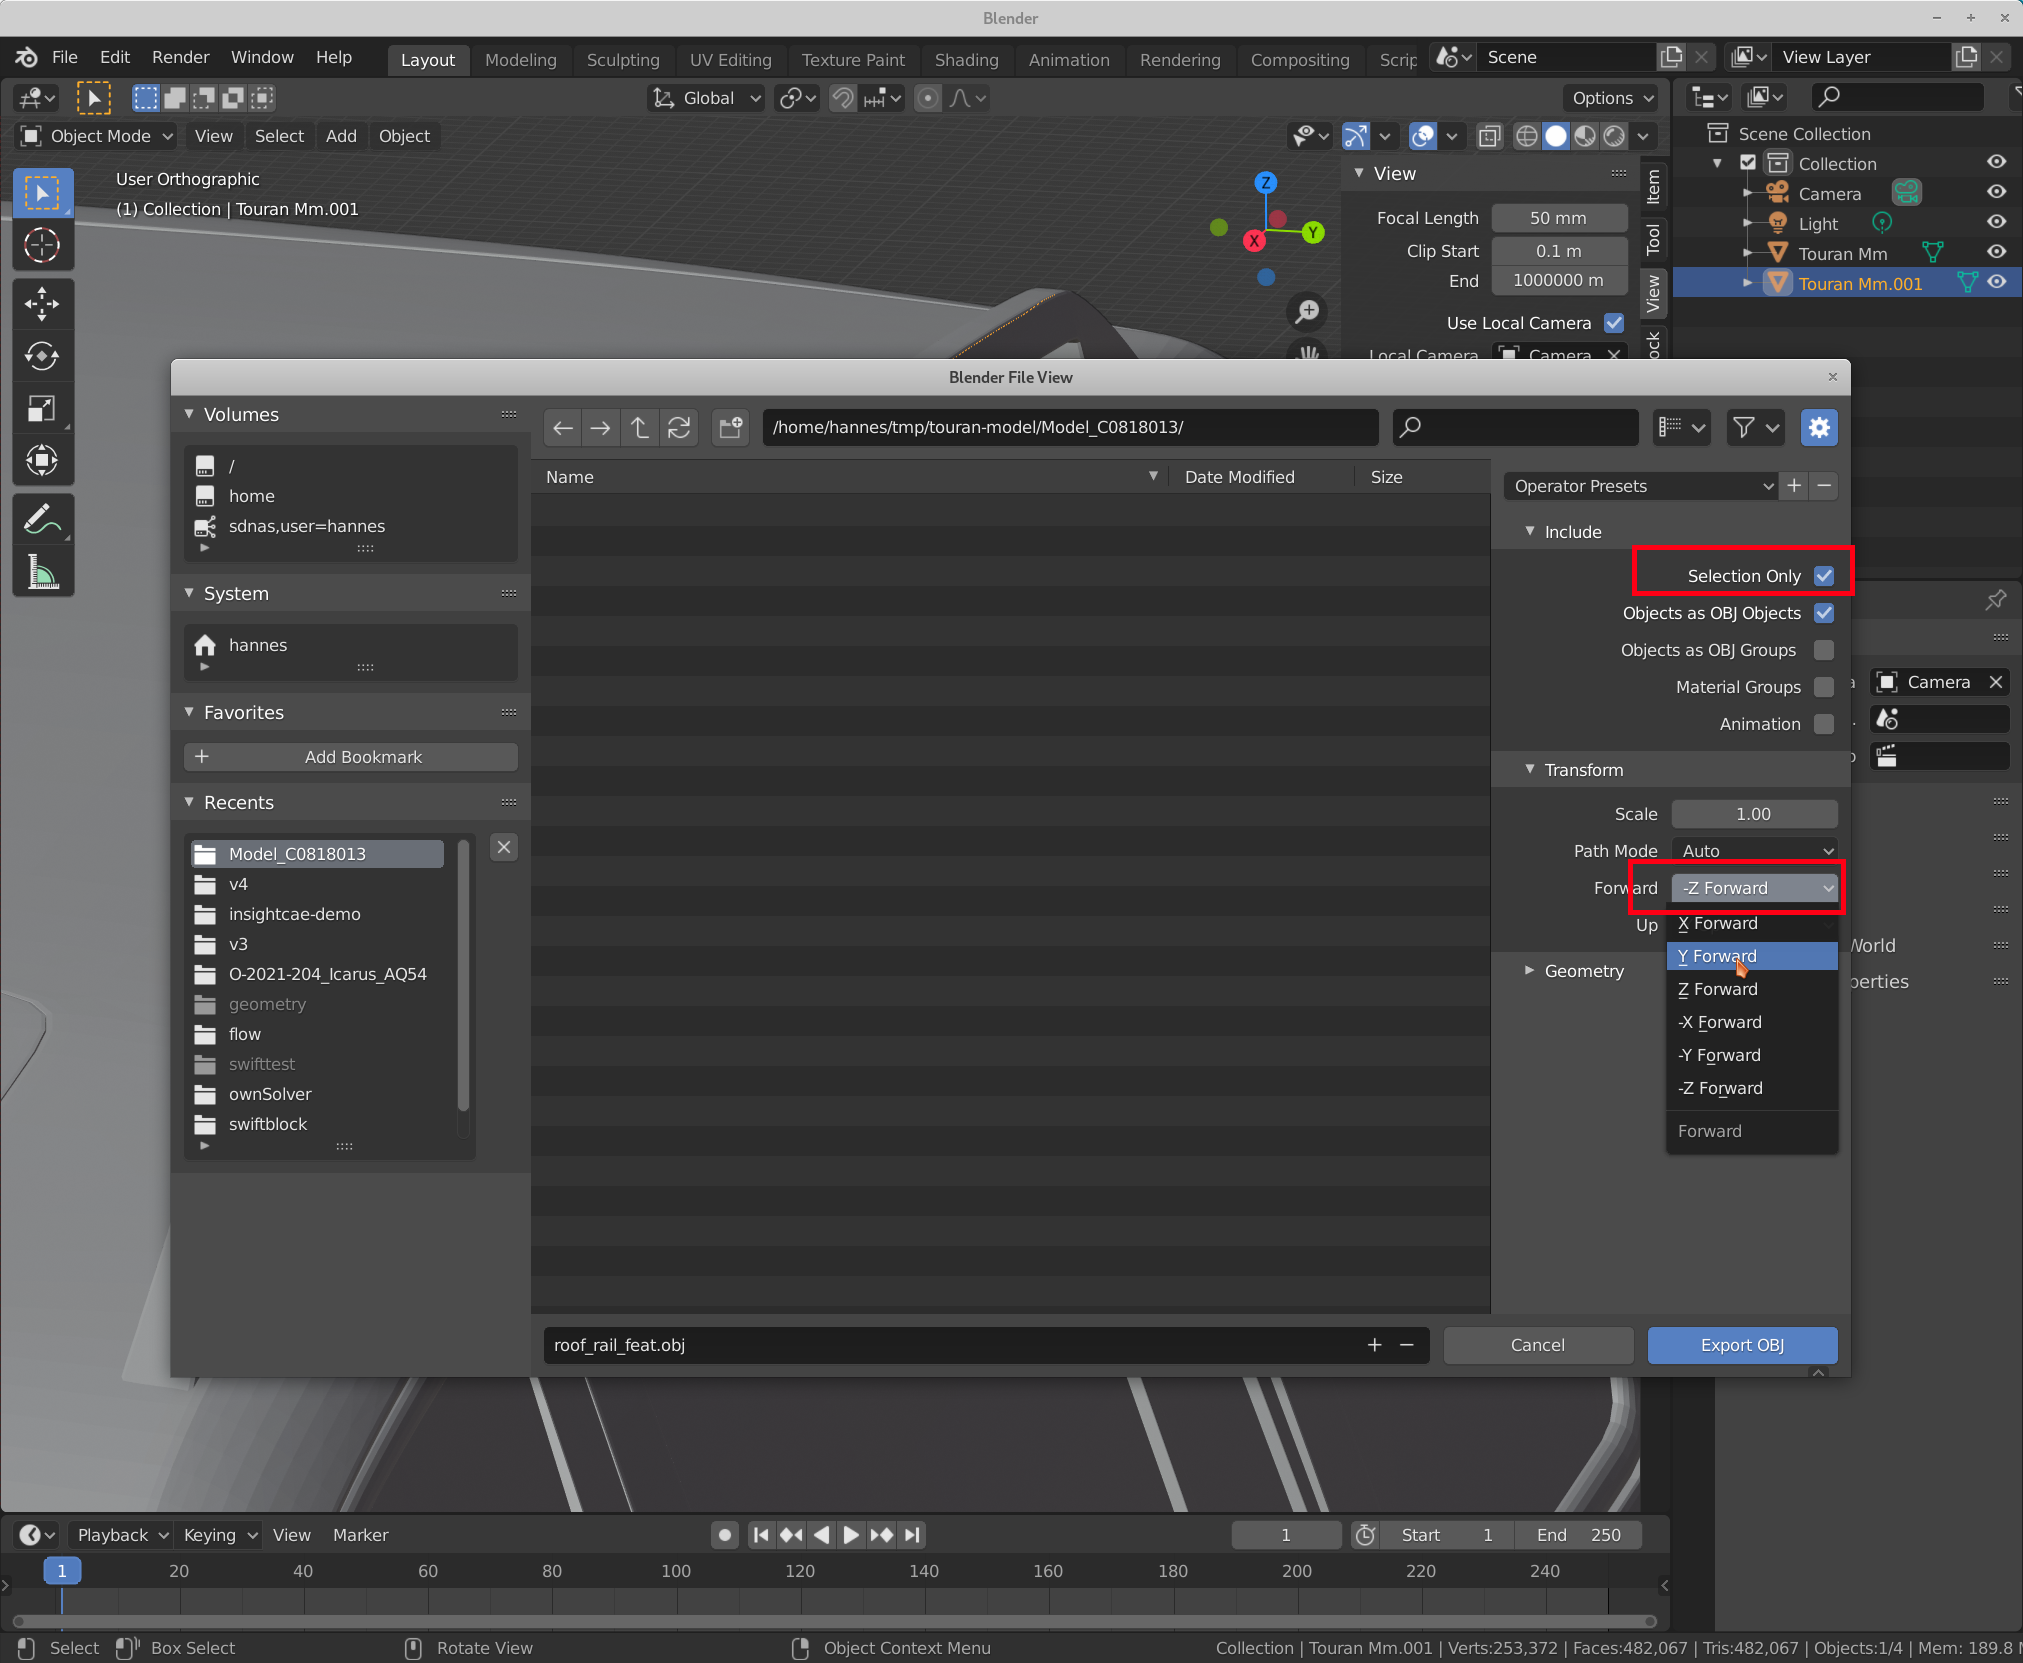
\includegraphics[width=0.75\linewidth]{figs/feature_edges_blender/11_export_setup}

\item the resulting OBJ files can be loaded into Paraview and checked

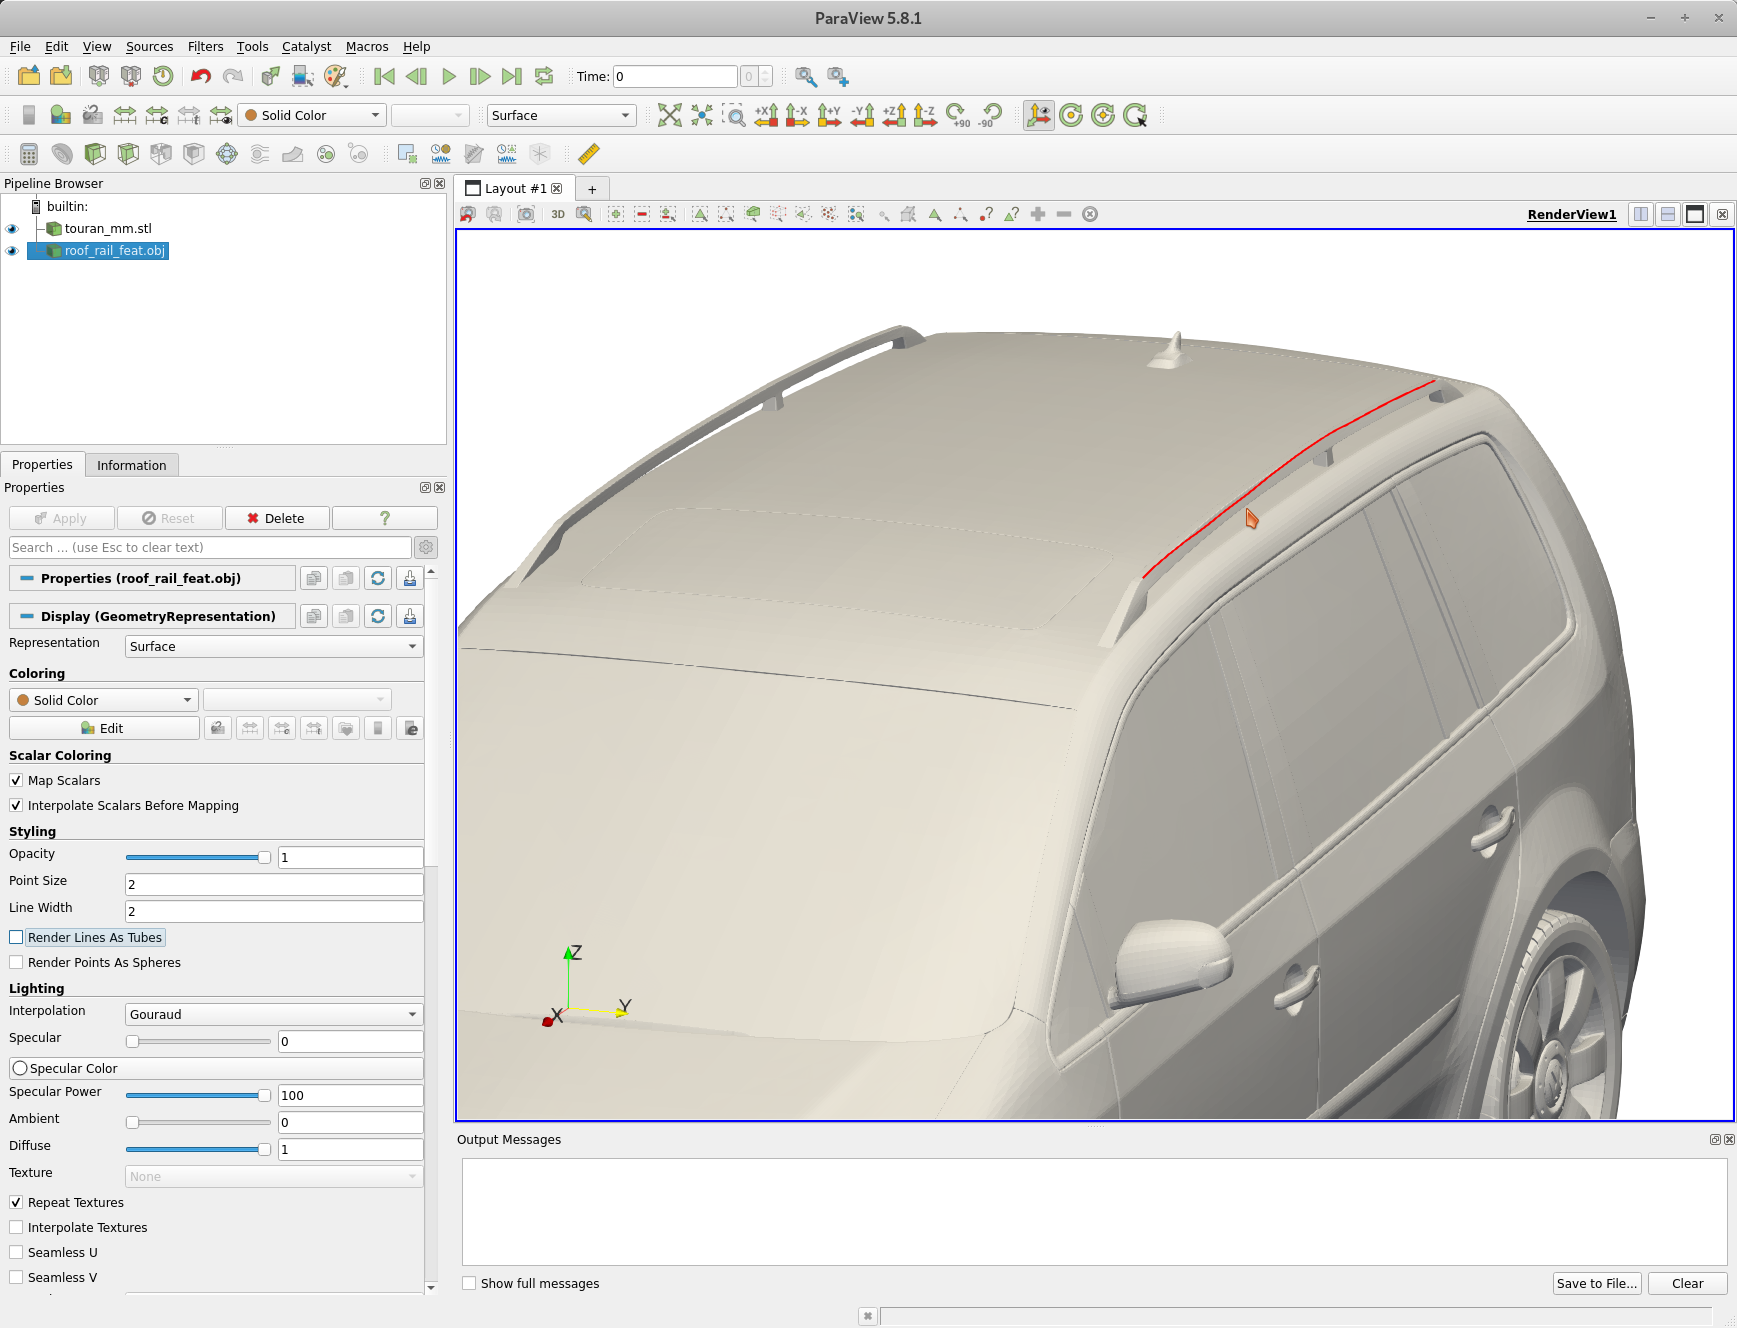
\includegraphics[width=0.75\linewidth]{figs/feature_edges_blender/12_view_paraview}

\item Finally, the OBJ files can be converted into OpenFOAM's eMesh format.
There is a tool called "surfaceFeatureConvert" in the OpenFOAM toolbox, which can perform this task.
The file type is recognized from the extension.
If not already done, the OpenFOAM environment needs to be loaded (here using the alias of1806):

\begin{lstlisting}
$ of1806
$ surfaceFeatureConvert roof_rail_feat.obj roof_rail_feat.eMesh
\end{lstlisting}


\end{enumerate}
